% Options for packages loaded elsewhere
\PassOptionsToPackage{unicode}{hyperref}
\PassOptionsToPackage{hyphens}{url}
%
\documentclass[
]{book}
\usepackage{amsmath,amssymb}
\usepackage{lmodern}
\usepackage{iftex}
\ifPDFTeX
  \usepackage[T1]{fontenc}
  \usepackage[utf8]{inputenc}
  \usepackage{textcomp} % provide euro and other symbols
\else % if luatex or xetex
  \usepackage{unicode-math}
  \defaultfontfeatures{Scale=MatchLowercase}
  \defaultfontfeatures[\rmfamily]{Ligatures=TeX,Scale=1}
\fi
% Use upquote if available, for straight quotes in verbatim environments
\IfFileExists{upquote.sty}{\usepackage{upquote}}{}
\IfFileExists{microtype.sty}{% use microtype if available
  \usepackage[]{microtype}
  \UseMicrotypeSet[protrusion]{basicmath} % disable protrusion for tt fonts
}{}
\makeatletter
\@ifundefined{KOMAClassName}{% if non-KOMA class
  \IfFileExists{parskip.sty}{%
    \usepackage{parskip}
  }{% else
    \setlength{\parindent}{0pt}
    \setlength{\parskip}{6pt plus 2pt minus 1pt}}
}{% if KOMA class
  \KOMAoptions{parskip=half}}
\makeatother
\usepackage{xcolor}
\IfFileExists{xurl.sty}{\usepackage{xurl}}{} % add URL line breaks if available
\IfFileExists{bookmark.sty}{\usepackage{bookmark}}{\usepackage{hyperref}}
\hypersetup{
  pdftitle={Foundations of Biology and Environmental Science: An Open-Access Encyclepedia},
  pdfauthor={Compiled and edited by Nathan Brouwer},
  hidelinks,
  pdfcreator={LaTeX via pandoc}}
\urlstyle{same} % disable monospaced font for URLs
\usepackage{longtable,booktabs,array}
\usepackage{calc} % for calculating minipage widths
% Correct order of tables after \paragraph or \subparagraph
\usepackage{etoolbox}
\makeatletter
\patchcmd\longtable{\par}{\if@noskipsec\mbox{}\fi\par}{}{}
\makeatother
% Allow footnotes in longtable head/foot
\IfFileExists{footnotehyper.sty}{\usepackage{footnotehyper}}{\usepackage{footnote}}
\makesavenoteenv{longtable}
\usepackage{graphicx}
\makeatletter
\def\maxwidth{\ifdim\Gin@nat@width>\linewidth\linewidth\else\Gin@nat@width\fi}
\def\maxheight{\ifdim\Gin@nat@height>\textheight\textheight\else\Gin@nat@height\fi}
\makeatother
% Scale images if necessary, so that they will not overflow the page
% margins by default, and it is still possible to overwrite the defaults
% using explicit options in \includegraphics[width, height, ...]{}
\setkeys{Gin}{width=\maxwidth,height=\maxheight,keepaspectratio}
% Set default figure placement to htbp
\makeatletter
\def\fps@figure{htbp}
\makeatother
\setlength{\emergencystretch}{3em} % prevent overfull lines
\providecommand{\tightlist}{%
  \setlength{\itemsep}{0pt}\setlength{\parskip}{0pt}}
\setcounter{secnumdepth}{5}
\usepackage{booktabs}
\ifLuaTeX
  \usepackage{selnolig}  % disable illegal ligatures
\fi

\title{Foundations of Biology and Environmental Science: An Open-Access Encyclepedia}
\author{Compiled and edited by Nathan Brouwer}
\date{2021-09-03}

\begin{document}
\maketitle

{
\setcounter{tocdepth}{1}
\tableofcontents
}
\hypertarget{introduction}{%
\chapter{Introduction}\label{introduction}}

\hypertarget{a}{%
\chapter{A}\label{a}}

\hypertarget{alignments}{%
\section{Alignments}\label{alignments}}

From Sharber, W. \href{https://towardsdatascience.com/introduction-to-sequence-alignments-with-biopython-f3b6375095db}{Introduction to Sequence Alignments with Biopython}. Towards Data Science. Medium.
\url{https://towardsdatascience.com/introduction-to-sequence-alignments-with-biopython-f3b6375095db}

``When working with biological sequence data, either DNA, RNA, or protein, biologists often want to be able to compare one sequence to another in order to make some inferences about the function or evolution of the sequences. Just like you wouldn't want to use data from data tables where data was in the wrong column for analyses, in order to make robust inferences from sequence data, we need to make sure our sequence data is well organized or ``aligned.'' Unfortunately, sequence data does not come with nice labels, like a date, miles per gallon, or horsepower. Instead, all we have is the position number in the sequence, and that is relative to that sequence only. Luckily, many sequences are highly conserved or similar between related organisms (and all organisms are related to some degree!). If we're fairly certain that we've obtained data from the same sequence from multiple organisms, we can put that data into a matrix that we call an alignment. If you're only comparing two sequences, it's called a pairwise alignment. If you're comparing three or more sequences, it's called a multiple sequence alignment (MSA).

``Using the positions and the identity of each molecule in the sequence, we can infer the relative placement of each molecule in the matrix. Sometimes there will be differences in the sequence, for example, in a position where most sequences are C, we find a sequence with a G. This is referred to as a single nucleotide polymorphism (SNP). In other times, we find that a sequence is missing a molecule that is present in the rest, or a sequence has an extra molecule. The former is a deletion, while the latter is an insertion, together referred to as ``indels.'' When aligning sequences with indels, we must account for these extra or missing molecules by adding gaps to the remaining sequences. These small differences are usually the interesting parts of sequence data because the variation is how we can make inferences on the function or evolution of the sequence\ldots''

\hypertarget{talking-glossary-allele-0.5-min}{%
\section{Talking Glossary: Allele (0.5 min)}\label{talking-glossary-allele-0.5-min}}

Note: This glossary definition focuses on the traditional definition of an allele. More broadly, an allele is \emph{any} genetic variant, whether it is in coding or non-coding DNA, impacts the phenotype of an organism or is neutral, involves a single base or many. This is mentioned in the last line of the abstract.

\textbf{Abstract}: ``An allele is one of two or more versions of a gene {[}or, more generally, a locus{]}. An individual inherits two alleles for each gene {[}locus{]}, one from each parent. If the two alleles are the same, the individual is homozygous for that gene {[}locus{]}. If the alleles are different, the individual is heterozygous. \textbf{Though the term allele was originally used to describe variation among genes, it now also refers to variation among non-coding DNA sequences} {[}emphasis added{]}.''

Audio: \url{https://www.genome.gov/sites/default/files/tg/en/narration/allele.mp3}

Note Any time they say ``gene'', think ``locus.''

\textbf{Transcript}: ````Allele'' is the word that we use to describe the alternative form or versions of a gene. People inherit one allele for each autosomal gene {[}locus{]} from each parent, and we tend to lump the alleles into categories. Typically, we call them either normal or wild-type alleles, or abnormal, or mutant alleles.''

Leslie G. Biesecker, M.D.

Image (from)
\url{https://rarediseases.info.nih.gov/files/glossary/english/allele_sm.jpg}

\hypertarget{b}{%
\chapter{B}\label{b}}

\hypertarget{talking-glossary-bioinformatics}{%
\section{Talking glossary: Bioinformatics}\label{talking-glossary-bioinformatics}}

\url{https://www.genome.gov/genetics-glossary/Bioinformatics}

\textbf{Transcript}: ``Bioinformatics is a field of computational science that has to do with the analysis of sequences of biological molecules. {[}It{]} usually refers to genes, DNA, RNA, or protein, and is particularly useful in comparing genes and other sequences in proteins and other sequences within an organism or between organisms, looking at evolutionary relationships between organisms, and using the patterns that exist across DNA and protein sequences to figure out what their function is. You can think about bioinformatics as essentially the linguistics part of genetics. That is, the linguistics people are looking at patterns in language, and that's what bioinformatics people do--looking for patterns within sequences of DNA or protein.''

Christopher P. Austin, M.D.

\hypertarget{c}{%
\chapter{C}\label{c}}

\hypertarget{clade}{%
\section{Clade}\label{clade}}

Adapted from Wikipedia
\url{https://en.wikipedia.org/wiki/Clade}

A clade, also known as a monophyletic group, is a group of organisms that are monophyletic ---that is, composed of a common ancestor and all its descendants .{[}4{]} . The common ancestor may be an individual, a population , a species (extinct or extant ), and so on. Clades are nested, one in another, as each branch in turn splits into smaller branches. These splits reflect evolutionary history as populations diverged and evolved independently. The term ``clade'' is also used with a similar meaning in other fields besides biology, such as historical linguistics.

A clade is by definition monophyletic , meaning that it contains one ancestor (which can be an organism, a population, or a species) and all its descendants.{[}note 1{]} {[}12{]} {[}13{]} The ancestor can be known or unknown; any and all members of a clade can be extant or extinct.

\href{https://upload.wikimedia.org/wikipedia/commons/thumb/4/46/Clade-grade_II.svg/640px-Clade-grade_II.svg.png}{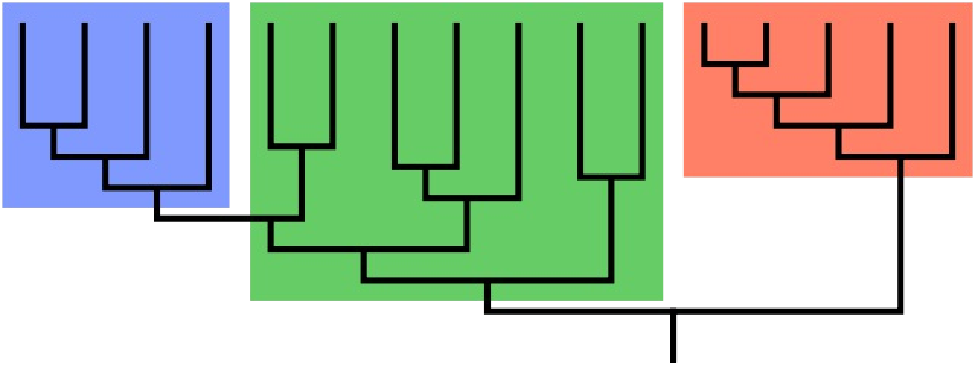
\includegraphics{openbio_files/figure-latex/unnamed-chunk-1-1.pdf}}

Over the last few decades, the cladistic approach has revolutionized biological classification and revealed surprising evolutionary relationships among organisms.{[}5{]} Taxonomists have worked to make the taxonomic system reflect evolution. Taxonomists therefore try to avoid naming taxa that are not clades; that is, taxa that are not monophyletic . Some of the relationships between organisms that the molecular biology arm of cladistics has revealed are that fungi are closer relatives to animals than they are to plants, archaea are now considered different from bacteria , and multicellular organisms may have evolved from archaea.{[}6{]}

\href{https://upload.wikimedia.org/wikipedia/commons/1/11/Cladogram_Crocodilia_NL.PNG}{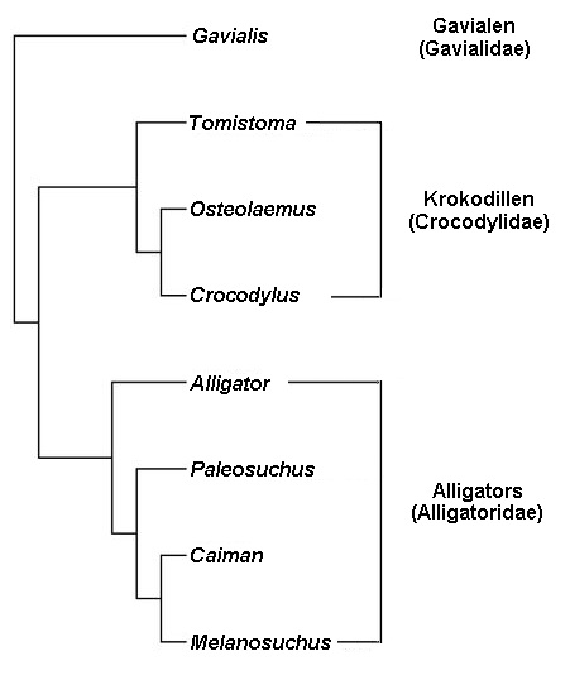
\includegraphics{openbio_files/figure-latex/unnamed-chunk-2-1.pdf}}

Many commonly named groups, rodents and insects for example, are clades because, in each case, the group consists of a common ancestor with all its descendant branches. Rodents, for example, are a branch of mammals that split off after the end of the period when the clade Dinosauria stopped being the dominant terrestrial vertebrates 66 million years ago. The original population and all its descendants are a clade. The rodent clade corresponds to the order Rodentia, and insects to the class Insecta. These clades include smaller clades, such as chipmunk or ant , each of which consists of even smaller clades. The clade ``rodent'' is in turn included in the mammal, vertebrate and animal clades.

\hypertarget{clades-and-phylogenetic-trees}{%
\subsection{Clades and phylogenetic trees}\label{clades-and-phylogenetic-trees}}

The science that tries to reconstruct phylogenetic trees and thus discover clades is called phylogenetics . The results of phylogenetic analyses are tree-shaped diagrams called phylogenies; they, and all their branches, are phylogenetic hypotheses.{[}14{]}

\hypertarget{terminology}{%
\subsection{Terminology}\label{terminology}}

The relationship between clades can be described in several ways:

\begin{enumerate}
\def\labelenumi{\arabic{enumi}.}
\tightlist
\item
  A clade located within a clade is said to be nested within that clade. In the diagram, the hominoid clade, i.e.~the apes and humans, is nested within the primate clade.
\item
  Two clades are sisters (sister groups sister clades) if they have an immediate common ancestor. In the diagram, lemurs and lorises are sister clades, while humans and tarsiers are not.
\end{enumerate}

\href{https://upload.wikimedia.org/wikipedia/commons/thumb/5/5e/Primate_cladogram.svg/556px-Primate_cladogram.svg.png}{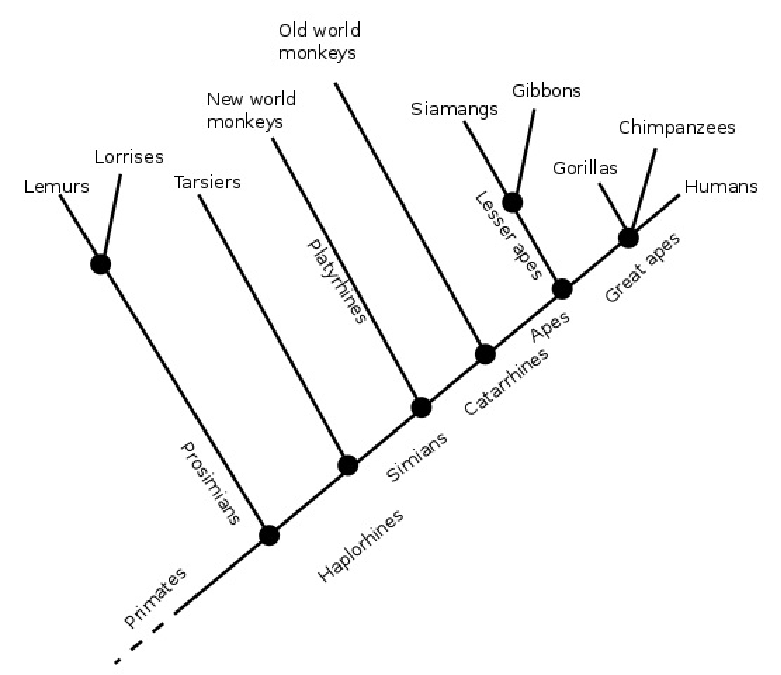
\includegraphics{openbio_files/figure-latex/unnamed-chunk-3-1.pdf}}

\hypertarget{in-popular-culture}{%
\section{In popular culture}\label{in-popular-culture}}

An episode of \href{https://en.wikipedia.org/wiki/Elementary_(TV_series)}{Elementary} is titled ``\href{https://en.wikipedia.org/wiki/List_of_Elementary_episodes\#ep38}{Dead Clade Walking}'' and deals with a case involving a rare fossil.

\hypertarget{references}{%
\subsection{References}\label{references}}

\begin{enumerate}
\def\labelenumi{\arabic{enumi}.}
\tightlist
\item
  Wells, John C. (2008). Longman Pronunciation Dictionary (3rd ed.). Longman. ISBN 978-1-4058-8118-0. ``clade''. Merriam-Webster Dictionary. Retrieved 19 April 2020.
  Martin, Elizabeth; Hin, Robert (2008). A Dictionary of Biology. Oxford University Press.
\item
  Cracraft, Joel; Donoghue, Michael J., eds.~(2004). ``Introduction''. Assembling the Tree of Life. Oxford University Press. p.~1. ISBN 978-0-19-972960-9.
\item
  Palmer, Douglas (2009). Evolution: The Story of Life. Berkeley: University of California Press. p.~13.
\item
  Pace, Norman R. (18 May 2006). ``Time for a change''. Nature. 441 (7091): 289. Bibcode:2006Natur.441..289P. \url{doi:10.1038/441289a}. ISSN 1476-4687. PMID 16710401. S2CID 4431143.
\item
  Dupuis, Claude (1984). ``Willi Hennig's impact on taxonomic thought''. Annual Review of Ecology and Systematics. 15: 1--24. \url{doi:10.1146/annurev.es.15.110184.000245}.
\item
  Huxley, J. S. (1957). ``The three types of evolutionary process''. Nature. 180 (4584): 454--455. Bibcode:1957Natur.180..454H. \url{doi:10.1038/180454a0}. S2CID 4174182.
\item
  Huxley, T.H. (1876): Lectures on Evolution. New York Tribune. Extra. no 36. In Collected Essays IV: pp 46-138 original text w/ figures
\item
  Brower, Andrew V. Z. (2013). ``Willi Hennig at 100''. Cladistics. 30 (2): 224--225. \url{doi:10.1111/cla.12057}.
\item
  ''Evolution 101''. page 10. Understanding Evolution website. University of California, Berkeley. Retrieved 26 February 2016.
\item
  ``International Code of Phylogenetic Nomenclature. Version 4c. Chapter I. Taxa''. 2010. Retrieved 22 September 2012.
\item
  Envall, Mats (2008). ``On the difference between mono-, holo-, and paraphyletic groups: a consistent distinction of process and pattern''. Biological Journal of the Linnean Society. 94: 217. \url{doi:10.1111/j.1095-8312.2008.00984.x}.
\item
  Nixon, Kevin C.; Carpenter, James M. (1 September 2000). ``On the Other''Phylogenetic Systematics''\,``. Cladistics. 16 (3): 298--318. \url{doi:10.1111/j.1096-0031.2000.tb00285.x}. S2CID 73530548.
\end{enumerate}

\hypertarget{talking-glossary-cloning-0.5-min}{%
\section{Talking Glossary: Cloning (0.5 min)}\label{talking-glossary-cloning-0.5-min}}

National Human Genome Research Institute
\url{https://www.genome.gov/genetics-glossary/Cloning}

\textbf{Introduction}: ``Cloning is the process of making identical copies of an organism, cell, or DNA sequence. Molecular cloning is a process by which scientists amplify a desired DNA sequence. The target sequence is isolated, inserted into another DNA molecule (known as a vector), and introduced into a suitable host cell. Then, each time the host cell divides, it replicates the foreign DNA sequence along with its own DNA. Cloning also can refer to asexual reproduction.''

Audio: \url{https://www.genome.gov/sites/default/files/tg/en/narration/cloning.mp3}

\textbf{Transcript}: ``Cloning is a word we use to describe a molecular process of making millions or billions of copies of a single molecule. It's different from the uses of the terms''cellular cloning'' or ``organism cloning'' that are used in the reproductive genetics universe. We use molecular cloning to amplify, or make many copies of, genes or proteins or other micro molecules that amplifies the signal and allows us to study these molecules in a laboratory''.

Leslie G. Biesecker, M.D.

\hypertarget{talking-glossary-codominance-0.5-min}{%
\section{Talking Glossary: Codominance (0.5 min)}\label{talking-glossary-codominance-0.5-min}}

Abstract: ``Codominance is a relationship between two versions of a gene. Individuals receive one version of a gene, called an allele, from each parent. If the alleles are different, the dominant allele usually will be expressed, while the effect of the other allele, called recessive, is masked. In codominance, however, neither allele is recessive and the phenotypes of both alleles are expressed.''

Audio: \url{https://www.genome.gov/sites/default/files/tg/en/narration/codominance.mp3}

Image: \url{https://www.genome.gov/sites/default/files/tg/en/illustration/codominance.jpg}
Transcript

Codominance means that neither allele can mask the expression of the other allele. An example in humans would be the ABO blood group, where alleles A and alleles B are both expressed. So if an individual inherits allele A from their mother and allele B from their father, they have blood type AB.

\href{https://www.genome.gov/staff/Suzanne-Hart-PhD}{Suzanne Hart}, Ph.D.

\hypertarget{comparative-genomics}{%
\section{Comparative genomics}\label{comparative-genomics}}

Adapted from Wikipedia

\url{https://en.wikipedia.org/wiki/Comparative_genomics}

Comparative genomics is a field of biological research in which the genomic features of different organisms are compared.{[}2{]}{[}3{]} The genomic features may include the DNA sequence, genes, gene order, regulatory sequences, and other genomic structural landmarks.{[}3{]} In this branch of genomics, whole genomes resulting from genome projects are compared to study basic biological similarities and differences as well as evolutionary relationships between organisms.{[}2{]}{[}4{]}{[}5{]} The major principle of comparative genomics is that common features of two organisms will often be encoded within the DNA that is evolutionarily conserved between them.{[}6{]} Therefore, comparative genomic approaches start with making some form of alignment of genome sequences and looking for similar sequences in the aligned genomes and checking to what extent those sequences are conserved. Based on these, genome and molecular evolution are inferred and this may, in turn, be put in the context of, for example, evolution, ecology, or pathogenicity.

Comparative genomics is now a standard component of the analysis of every new genome sequence.{[}2{]}{[}8{]} With the explosion in the number of genome projects due to the advancements in DNA sequencing technologies{[}9{]} Comparative genomics has revealed high levels of similarity between closely related organisms, such as humans and chimpanzees, and, more surprisingly, similarity between seemingly distantly related organisms, such as humans and yeast.

The medical field benefits from the study of comparative genomics. Vaccine development in particular has experienced useful advances in technology due to genomic approaches to problems. In an approach known as reverse vaccinology, researchers can discover candidate antigens (proteins in pathogens that can be targeted by the immune system) for vaccine development by analyzing the genome of a pathogen or a family of pathogens.

1* Darling A.E.; Miklós I.; Ragan M.A.~(2008). ``Dynamics of Genome Rearrangement in Bacterial Populations''. PLOS Genetics. 4 (7): e1000128. \url{doi:10.1371/journal.pgen.1000128}. PMC 2483231. PMID 18650965. open access
1. Touchman, J. (2010). ``Comparative Genomics''. Nature Education Knowledge. 3 (10): 13.
1. Xia, X. (2013). Comparative Genomics. SpringerBriefs in Genetics. Heidelberg: Springer. \url{doi:10.1007/978-3-642-37146-2}. ISBN 978-3-642-37145-5. S2CID 5491782.
1. Russel, P.J.; Hertz, P.E.; McMillan, B. (2011). Biology: The Dynamic Science (2nd ed.). Belmont, CA: Brooks/Cole. pp.~409--410.
1. Primrose, S.B.; Twyman, R.M. (2003). Principles of Genome Analysis and Genomics (3rd ed.). Malden, MA: Blackwell Publishing.
1. Hardison, R.C. (2003). ``Comparative genomics''. PLOS Biology. 1 (2): e58. \url{doi:10.1371/journal.pbio.0000058}. PMC 261895. PMID 14624258. open access
1. Ellegren, H. (2008). ``Comparative genomics and the study of evolution by natural selection''. Molecular Ecology. 17 (21): 4586--4596. \url{doi:10.1111/j.1365-294X.2008.03954.x}. PMID 19140982. S2CID 43171654.
1. Koonin, E.V.; Galperin, M.Y. (2003). Sequence - Evolution - Function: Computational approaches in comparative genomics. Dordrecht: Springer Science+Business Media.

\hypertarget{talking-glossary-contig-0.75-min}{%
\section{Talking Glossary: Contig (0.75 min)}\label{talking-glossary-contig-0.75-min}}

\url{https://www.genome.gov/genetics-glossary/Contig}

\textbf{Abstract}: ``A contig--from the word''contiguous''--is a series of overlapping DNA sequences used to make a physical map that reconstructs the original DNA sequence of a chromosome or a region of a chromosome. A contig can also refer to one of the DNA sequences used in making such a map.''

Audio: \url{https://www.genome.gov/sites/default/files/tg/en/narration/contig.mp3}

Image: \url{https://www.genome.gov/sites/default/files/tg/en/narration/contig.mp3}

\textbf{Transcript}: ``A chromosome is a very long molecule of DNA. And it is very hard to study it at once, so what researchers do is they break it into smaller pieces and they sequence each one of those individual pieces first, and then they attempt to put it together to reconstruct the original chromosome sequence. A contig is the physical map, which results from putting together several little overlapping bits of DNA into a longer sequence. The contig is the physical map resulting from taking small pieces of DNA that overlap and putting them together into a longer sequence.''

\href{https://www.genome.gov/staff/Belen-Hurle-PhD}{Belen Hurle}, Ph.D.

\hypertarget{talking-glossary---foundations-1-review-crossing-over}{%
\section{Talking Glossary - Foundations 1 Review: Crossing over}\label{talking-glossary---foundations-1-review-crossing-over}}

Abstract: ``Crossing over is the swapping of genetic material that occurs in the germ line. During the formation of egg and sperm cells, also known as meiosis, paired chromosomes from each parent align so that similar DNA sequences from the paired chromosomes cross over one another. Crossing over results in a shuffling of genetic material and is an important cause of the genetic variation seen among offspring.''

Audio:
\url{https://www.genome.gov/sites/default/files/tg/en/narration/crossing_over.mp3}

\textbf{Transcript}: ``Crossing over is a biological occurrence that happens during meiosis when the paired homologs, or chromosomes of the same type, are lined up. In meiosis, they're lined up on the meiotic plates, {[}as they're{]} sometimes called, and those paired chromosomes then have to have some biological mechanism that sort of keeps them together. And it turns out that there are these things called chiasmata, which are actually where strands of the duplicated homologous chromosomes break and recombine with the same strand of the other homolog. So if you have two Chromosome 1s lined up, one strand of one Chromosome 1 will break and it will reanneal with a similar breakage on the other Chromosome 1. So that then the new chromosome that will happen will have part of, say, the maternal Chromosome 1 and the paternal Chromosome 1, where maternal and paternal means where that person got their Chromosomes 1s from, their one or their two. Therefore, the child that's formed out of one of those Chromosome 1s now has a piece of his or her grandmother's Chromosome 1 and a piece of his or her grandfather's Chromosome 1. And it's this crossing over that lets recombination across generations of genetic material happen, and it also allows us to use that information to find the locations of genes.''

\href{https://www.genome.gov/staff/Joan-E-Bailey-Wilson-PhD}{Joan E. Bailey-Wilson}, Ph.D

Photo: \url{https://i.irp.nih.gov/pi/0010100622.jpg}

\hypertarget{d}{%
\chapter{D}\label{d}}

\hypertarget{talking-glossary-deletion-mutation-1.5-min}{%
\section{Talking Glossary: Deletion mutation (1.5 min)}\label{talking-glossary-deletion-mutation-1.5-min}}

\url{https://www.genome.gov/genetics-glossary/Deletion}

\textbf{Abstract}: ``Deletion is a type of mutation involving the loss of genetic material. It can be small, involving a single missing DNA base pair, or large, involving a piece of a chromosome.''

Note: Among evolutionary biologists, ``deletion'' usually means deletion of a single base; larger deletions are specified, e.g.~``chromosomal deletion.'' In order to recognize a deletion, there's needs to be some frame of reference, such as a consensus sequence, a reference genomic sequence, or other individuals in a multiple sequence alignment (MSA). Deletions of all sizes can be useful for constructing phylogenies.

Image: \url{https://www.genome.gov/sites/default/files/tg/en/illustration/deletion.jpg}
Example of single base and chromosomal deletion.

\textbf{Transcript:} ``Deletion really means that something is missing. And as a geneticist talking about deletion it means something is missing of the genetic material. And it can be something small, just a base pair; it can be something larger; it can be part of a gene; it can be even larger; it can be an entire gene; or yet larger again, it can be part of the chromosome. And depending upon what it is, you have to look at it in different ways. You can find a deletion in a chromosome just by doing a cytogenetic or chromosome analysis, or a deletion in a gene you can find out by sequencing the DNA. So when you have a deletion, depending upon the size, it can have different effects. What was the most surprising to me was that just by having a deletion of one base pair, you can have the most severe birth defect, and sometimes by missing an entire chromosome, you don't even see all that much compared to just having a deletion of a small base pair. Different deletions can lead to different findings, and they can affect just behavior; they can affect how a child, how a person looks; they can affect a very severe problem that the child may die at birth; or they can affect something that just has to do with eye color, hair color, with weight or height of the person.''

Maximilian Muenke, M.D.

\hypertarget{talking-glossary-dna-sequencing-0.75-min}{%
\section{Talking Glossary: DNA sequencing (0.75 min)}\label{talking-glossary-dna-sequencing-0.75-min}}

\textbf{Introduction}: ``DNA sequencing is a laboratory technique used to determine the exact sequence of bases (A, C, G, and T) in a DNA molecule. The DNA base sequence carries the information a cell needs to assemble protein and RNA molecules. DNA sequence information is important to scientists investigating the functions of genes. The technology of DNA sequencing was made faster and less expensive as a part of the Human Genome Project.''

\textbf{Transcript:} ``DNA consists of a linear string of nucleotides, or bases, for simplicity, referred to by the first letters of their chemical names--A, T, C and G. The process of deducing the order of nucleotides in DNA is called DNA sequencing. Since the DNA sequence confers information that the cell uses to make RNA molecules and proteins, establishing the sequence of DNA is key for understanding how genomes work. The technology for DNA sequencing was made faster and less expensive as a part of the Human Genome Project. And recent developments have profoundly increased the efficiency of DNA sequencing even further.''

Eric D. Green, M.D., Ph.D.

\hypertarget{sex-chromosome-dosage-compensation}{%
\section{Sex-Chromosome Dosage compensation}\label{sex-chromosome-dosage-compensation}}

\href{https://en.wikipedia.org/wiki/Sex-Chromosome_Dosage_compensation}{Adapted from Wikipedia}

Dosage compensation is the process by which organisms equalize the expression of genes between individuals with different sex chromosome karyotypes (e.g.~XX versus XY). Across species, different ``sexes'' are often characterized by different types and numbers of sex chromosomes . In order to neutralize the large difference in gene dosage produced by differing numbers of sex chromosomes, various evolutionary branches have acquired various methods to equalize gene expression . Because sex chromosomes contain different numbers of genes , different species of organisms have developed different mechanisms to cope with this inequality. Replicating the actual gene is impossible; thus organisms instead equalize the expression from each gene. For example, in humans , XX individuals silence the transcription of one X chromosome of each pair, and transcribe all information from the other, expressed X chromosome. Thus, human XX individuals have the same number of expressed X-linked genes as do human XY individuals, with both having essentially one X chromosome per cell, from which to transcribe and express genes. This is called X-inactivation. In each XX cell, one of the two X chromosomes is randomly inactivated.

Other lineages have evolved different mechanisms to cope with the differences in gene copy numbers between the sexes that are observed on sex chromosomes. Some lineages have evolved upregulation mechanisms which restores expression of X-specific genes in the heterogametic sex (e.g.~XY) to the same levels observed in the ancestor prior to the evolution of the sex chromosome.

\hypertarget{random-inactivation-of-one-x-in-xx-individuals}{%
\subsection{Random inactivation of one X in XX individuals}\label{random-inactivation-of-one-x-in-xx-individuals}}

One logical way to equalize gene expression amongst XX and XY that follow a XX/XY sex differentiation scheme would be to decrease or altogether eliminate the expression of one of the X chromosomes in an XX, (homogametic) individual, such that both XX and XY individuals express only one X chromosome. This is the case in many mammalian organisms, including humans and mice.{[}1 This process involves histone tail modifications, DNA methylation patterns, and reorganization of large-scale chromatin structure. In spite of these extensive modifications, not all genes along the X chromosome are subject to X-inactivation.

\hypertarget{two-fold-increased-transcription-of-a-single-x-in-xy-individuals}{%
\subsection{Two-fold increased transcription of a single X in XY individuals}\label{two-fold-increased-transcription-of-a-single-x-in-xy-individuals}}

Another mechanism common for achieving equal X-related genetic expression between XX and XY indviduals involves two-fold increased transcription of a single X chromosome in XY individuals. Thus, heterogametic organisms (XY) with one X chromosome may match the level of expression achieved in homogametic individuals with two active X chromosomes. This mechanism is observed in Drosophila.

\hypertarget{talking-glossary-duplication-0.75-min}{%
\section{Talking Glossary: Duplication (0.75 min)}\label{talking-glossary-duplication-0.75-min}}

\textbf{Abstract}: ``Duplication is a type of mutation that involves the production of one or more copies of a gene or region of a chromosome. Gene and chromosome duplications occur in all organisms, though they are especially prominent among plants. Gene duplication is an important mechanism by which evolution occurs.''

Note: in introductory biology courses we typically focus on duplication of large portions of chromosomes or duplication of entire chromosmes.

Image: \url{https://www.genome.gov/sites/default/files/tg/en/illustration/duplication.jpg}

Audio: \url{https://www.genome.gov/sites/default/files/tg/en/narration/duplication.mp3}

Transcript: ``Duplications occur when there is more than one copy of a specific stretch of DNA. This can occur in several different contexts. During a disease process, extra copies of the gene can contribute to a cancer. Genes can also duplicate through evolution, where one copy can continue the original function and the other copy of the gene produces a new function. On occasion, whole chromosomes are duplicated. In humans this causes disease. Throughout evolution, there have been several occasions, both in fish and plants, where whole genomes have been duplicated.''

Lawrence C. Brody, Ph.D.

\hypertarget{b-1}{%
\chapter{B}\label{b-1}}

\hypertarget{talking-glossary-epigenetics}{%
\section{Talking Glossary: Epigenetics}\label{talking-glossary-epigenetics}}

\url{https://www.genome.gov/genetics-glossary/Epigenetics}

\textbf{Abstract}: Epigenetics is an emerging field of science that studies heritable changes caused by the activation and deactivation of genes without any change in the underlying DNA sequence of the organism. The word epigenetics is of Greek origin and literally means over and above (epi) the genome.

Audio: \url{https://www.genome.gov/sites/default/files/tg/en/narration/epigenetics.mp3}

\textbf{Transcript}: ``Epigenetics is the study of changes in gene function that are heritable and that are not attributed to alterations of the DNA sequence. The term epi means above. It's a Greek prefix. It's also defined as on top of the basic DNA sequence. In general terms you can think of them like accent marks on words where the DNA is the language and the modifications are the accent marks. Epigenetic marks change the way genes are expressed. The promise of epigenetics is that it tells us about the cell, it's a way to define the cell that's different than just looking at gene expression levels. We could look at any kind of cell and it will have specialized epigenetic patterns. There are two types of modifications: DNA methylation and histone modification. DNA methylation goes awry in cancers so if we knew the normal pattern of methylation and then looked at the pattern of methylation in a tumor we could see what changes were taking place and we could see which genes were being affected.''

\href{https://www.genome.gov/staff/Laura-Elnitski-PhD}{Laura Elnitski}

Photograph: \url{https://i.irp.nih.gov/pi/0012009821.jpg}

\hypertarget{f}{%
\chapter{F}\label{f}}

\hypertarget{talking-glossary-founder-effect-a-type-of-genetic-bottleneck-1-min}{%
\section{Talking glossary: Founder effect (A type of genetic bottleneck; 1 min)}\label{talking-glossary-founder-effect-a-type-of-genetic-bottleneck-1-min}}

\url{https://www.genome.gov/genetics-glossary/Founder-Effect}

\textbf{Abstract}: ``The founder effect is the reduction in genetic variation that results when a small subset of a large population is used to establish a new colony. The new population may be very different from the original population, both in terms of its genotypes and phenotypes. In some cases, the founder effect plays a role in the emergence of new species.''

Audio: \url{https://www.genome.gov/sites/default/files/tg/en/narration/founder_effect.mp3}

\textbf{Transcript}: ``Founder effect is a phenomenon in the work that we do that refers to the migration of a small group of people from a larger population to go settle in another environment. And they carry along with them a subset of genetic information that existed in the larger population. And because of that, carrying the subset, they actually reduce the amount of genetic variation that exists within a new population now. And as a result of that, they may emphasize certain phenotypes or certain genes, and all this may be deemphasized. So a founder effect can sometimes impact a population in such a way that they may have less of a particular type of gene or more of a particular type of gene. And it can change what we call phenotype, which is the things that we look at like your height, you know, your weight, or having a particular disease or not having a particular disease. So in effect that is what founder effect is.''

\href{https://en.wikipedia.org/wiki/Charles_Rotimi}{Charles N. Rotimi}, Ph.D.~is the Director of the Trans-National Institutes of Health (NIH) center for research in genomics and global health. He works to ensure that population genetics include genomes from African populations and founded the African Society of Human Genetics in 2003. Rotimi was instrumental in the launch of the Human Heredity and Health in Africa (H3Africa) with the NIH and the Wellcome Trust. He was elected to the National Academy of Medicine in 2018. (\href{https://en.wikipedia.org/wiki/Charles_Rotimi}{Wikipedia}))

Image: \url{https://upload.wikimedia.org/wikipedia/commons/thumb/a/a5/Charles_Rotimi_in_NHGRI\%27s_Oral_History_Collection.jpg/440px-Charles_Rotimi_in_NHGRI\%27s_Oral_History_Collection.jpg}

For an \href{https://www.genome.gov/player/H6tg-48aVP4/PL1ay9ko4A8sk0o9O-YhseFHzbU2I2HQQp}{interview} with Dr.~Rotimi see: \url{https://www.genome.gov/player/H6tg-48aVP4/PL1ay9ko4A8sk0o9O-YhseFHzbU2I2HQQp}

\hypertarget{talking-glossary-frameshift-mutation-1.5-min}{%
\section{Talking Glossary: Frameshift mutation (1.5 min)}\label{talking-glossary-frameshift-mutation-1.5-min}}

Abstract: ``A frameshift mutation is a type of mutation involving the insertion or deletion of a nucleotide in which the number of deleted base pairs is not divisible by three.''Divisible by three'' is important because the cell reads a gene in groups of three bases. Each group of three bases corresponds to one of 20 different amino acids used to build a protein. If a mutation disrupts this reading frame, then the entire DNA sequence following the mutation will be read incorrectly.''

Audio: \url{https://www.genome.gov/sites/default/files/tg/en/narration/frameshift_mutation.mp3}

Transcript

``A frameshift mutation is a particular type of mutation that involves either insertion or deletion of extra bases of DNA. Now, what's important here is the number three. The number of bases that are either added or subtracted can't be divisible by three. And that's important because the cell reads a gene in groups of three bases. Every group of three bases corresponds to one of the 20 different amino acids that are used by your body to make proteins. And keep in mind your body has a lot of proteins; everything from the material that makes up your skin, to the material that makes up your hair, to the digestive juices that help you digest that yummy lunch you just had. If a mutation disrupts one of those reading frames, so that the wrong amino acid is put in place, then the entire DNA sequence following the mutation will be disrupted or read incorrectly. Very often, what we see is a premature termination. Instead of the encoded protein being of a certain particular size, it'll end up being much shorter, and it won't be able to accomplish the role that's been set out for it.''

\href{https://irp.nih.gov/pi/elaine-ostrander}{Elaine A. Ostrander}, Ph.D.
Photo: \url{https://i.irp.nih.gov/pi/0011756295.jpg}

(see below for an optional video on Dr.~Ostrander's work on dog genomics)

Elaine A. Ostrander

Image
\url{https://www.genome.gov/sites/default/files/tg/en/illustration/frameshift_mutation.jpg}
Normal versus frameshift mutations
Frameshift mutations

Here's an optional video about Dr.~Ostrander's work on dog genomics:
\url{https://youtu.be/Tma8RdXADmU}

\hypertarget{g}{%
\chapter{G}\label{g}}

\hypertarget{talking-glossary-u03-gel-electrophoresis-3-min}{%
\section{Talking Glossary U03: Gel Electrophoresis (``3 min)}\label{talking-glossary-u03-gel-electrophoresis-3-min}}

AKA ``running a gel

National Human Genome Research Institute
\url{https://www.genome.gov/genetics-glossary/Electrophoresis}

Abstract: ``Electrophoresis is a laboratory technique used to separate DNA, RNA, or protein molecules based on their size and electrical charge. An electric current is used to move molecules to be separated through a gel. Pores in the gel work like a sieve, allowing smaller molecules to move faster than larger molecules. The conditions used during electrophoresis can be adjusted to separate molecules in a desired size range.''

Audio: \url{https://www.genome.gov/sites/default/files/tg/en/narration/electrophoresis.mp3}

Image (Wikipedia): \url{https://upload.wikimedia.org/wikipedia/commons/thumb/a/a6/Gel_electrophoresis_apparatus.JPG/188px-Gel_electrophoresis_apparatus.JPG}

\textbf{Transcript}: Electrophoresis is a very broadly used technique which, fundamentally, applies electric current to biological molecules, whether--they're usually DNA, they can be protein or RNA, too\ldots and separates these fragments into pieces which are larger or smaller. It's used in a variety of applications\ldots{} Everything from forensics for determining the identity of individuals that may have been involved in a crime, by linking their DNA pattern, their electrophoresis pattern, to one that's in a database. The whole basis by which the human genome was done is by something called capillary electrophoresis, by separating DNA into shorter pieces and then running them on these electrophoresis gels which allow the patterns of As, Cs, Ts, and Gs to be elucidated. They're also very important in protein research, and then genetic mutation research, because when proteins or DNA are mutated, they are frequently longer or shorter, and they therefore show up on an electrophoresis gel differently than normal, so many diagnostic tests are still done using electrophoresis, so it's a very widely used basic research technique, was very important for the understanding of gene and protein function, but it's now gotten into the area of clinical diagnostics and forensics as well. Electrophoresis is usually done in what looks like a box which has a positive charge at one end and a negative charge at the other. And as we all learned in basic physics, when you put a charged molecule into an environment like that, the negative molecules go to the positive charge, and vice versa. In looking at proteins in a gel, in one of these boxes, you usually take the entire protein, and you're looking at the entire length of the protein and seeing how big it is, and the bigger it is, the shorter it will migrate into the gel, so that the small proteins will end up at the bottom of the gel, because they have migrated the farthest, and the biggest ones will wind up staying at the top. In the case of DNA, DNA's a very long molecule, so you wouldn't want to run, for the most part, a whole DNA molecule from a cell onto a gel. It's just so big that it would never get into the gel, so what scientists do, and what people do in classrooms these days, is to chop up that DNA using things like inscription enzymes, which chop up the DNA into more manageable pieces in a reproducible way. And then those pieces, depending on how big the pieces are, migrate more or less into the gel father down the box from top to the bottom.

Christopher P. Austin, M.D.

\hypertarget{talking-glossary-gene-amplification-1.5-min}{%
\section{Talking Glossary: Gene amplification (1.5 min)}\label{talking-glossary-gene-amplification-1.5-min}}

National Human Genome Research Institute

\textbf{Introduction}: ``Gene amplification is an increase in the number of copies of a gene sequence. \ldots.. The term also can refer to polymerase chain reaction (PCR), a laboratory technique that is used by scientists to amplify gene sequences in a test tube.''

Note: Cloning and gene amplification are related concepts and are used interchangeably by some people. In this course its most important to know generally what the terms are referring to (increasing the number of copies of gene); there will not be a question where, for example ``cloning'' is a correct answer but ``gene amplification'' is wrong.

Audio: \url{https://www.genome.gov/sites/default/files/tg/en/narration/gene_amplification.mp3}

Transcript: ``Gene amplification is one of those clauses that means different things to different people, depending on how they look at it. At its simplest level, it means an increase in the number of copies of a gene sequence. Now, cancer cells sometimes make multiple copies of genes in response to erroneous signals from other cells or because of signals they're getting from the environment. So in that sense we think of it as a pretty negative term; it's heralding something that's not really supposed to have happened in the body that's clearly going on. But it's also just a very scientific term that doesn't have either a positive or a negative connotation. Because it refers to a laboratory technique called polymerase chain reaction, or PCR, and that's a technique which scientists can amplify a single gene in a test tube against the background of the three billion other bases that are floating around inside the test tube. That technique, PCR, or polymerase chain reaction, is really the backbone of a great deal of molecular biology that's being done today. As a matter of fact, the individual who discovered it ended up winning a Nobel Prize for it. So when you hear the phrase''gene amplification'', think first about the context, and then think about the specifics.''

\href{https://www.genome.gov/staff/Elaine-A-Ostrander-PhD}{Elaine A. Ostrander}, Ph.D.

\hypertarget{talking-glossary-gene-pool-0.75-min}{%
\section{Talking Glossary: Gene Pool (0.75 min)}\label{talking-glossary-gene-pool-0.75-min}}

\url{https://www.genome.gov/genetics-glossary/Gene-Pool} (Links to an external site.)

\textbf{Abstract}: ``A gene pool is the total genetic diversity found within a population or a species. A large gene pool has extensive genetic diversity and is better able to withstand the challenges posed by environmental stresses. Inbreeding contributes to the creation of a small gene pool and makes populations or species more likely to go extinct when faced with some type of stress.''

Audio: \url{https://www.genome.gov/sites/default/files/tg/en/narration/gene_pool.mp3}

\textbf{Transcript}: ``Gene pool refers to thorough genetic diversity that exists within a population {[}all of the genetic diversity{]}. The larger the genetic pool, the more the diversity and the more opportunity this population will have to survive environmental stress that may impact on them. So gene pool is really good in the sense that the larger the gene pool, the more the survival of that particular population in terms of withstanding different things that may come in terms of environment.''

\href{https://www.genome.gov/staff/Charles-N-Rotimi-PhD}{Charles N. Rotimi}, Ph.D

\hypertarget{gene-prediction}{%
\section{Gene prediction}\label{gene-prediction}}

\url{https://en.wikipedia.org/wiki/Gene_prediction}

In computational biology, gene prediction or gene finding refers to the process of identifying the regions of genomic DNA that encode genes. This includes protein-coding genes as well as RNA genes , but may also include prediction of other functional elements such as regulatory regions. Gene finding is one of the first and most important steps in understanding the genome of a species once it has been sequenced.

In its earliest days, ``gene finding'' was based on painstaking experimentation on living cells and organisms. Statistical analysis of the rates of homologous recombination of several different genes could determine their order on a certain chromosome , and information from many such experiments could be combined to create a genetic map specifying the rough location of known genes relative to each other. Today, with comprehensive genome sequence and powerful computational resources at the disposal of the research community, gene finding has been redefined as a largely computational problem.

Determining that a sequence is functional should be distinguished from determining the function of the gene or its product. Predicting the function of a gene and confirming that the gene prediction is accurate still demands \emph{in vivo} experimentation through gene knockout and other assays, although frontiers of bioinformatics research are making it increasingly possible to predict the function of a gene based on its sequence alone.

Gene prediction is one of the key steps in genome annotation , following sequence assembly , the filtering of non-coding regions and repeat masking.

Gene prediction is closely related to the so-called `target search problem' investigating how DNA-binding proteins (transcription factors ) locate specific binding sites within the genome. Many aspects of structural gene prediction are based on current understanding of underlying biochemical processes in the cell such as gene transcription , translation , protein--protein interactions and regulation processes , which are subject of active research in the various omics fields such as transcriptomics , proteomics , metabolomics , and more generally structural and functional genomics.

\hypertarget{genbank}{%
\section{GenBank}\label{genbank}}

From the blog post ``{[}Introduction to GenBank and Bioinformatics with Python{]}(\url{https://medium.com/@wvsharber/introduction-to-genbank-and-bioinformatics-with-python-8a25a0f15e3f}'' (Sharber 2015)

``GenBank {[}is{]} arguably one of the most important repositories of biological data in the world. GenBank, funded and operated by the National Institutes of Health (NIH) through the National Center for Biotechnology Information (NCBI), is a genetic sequence database. Researchers around the world submit their DNA sequences to GenBank to store and distribute them. Think of it as a huge library of DNA. Almost every DNA sequence that has ever been used in scientific research is stored in GenBank. Most academic publishers won't accept your manuscript without you submitting your DNA to GenBank. Talk about open-source data! In case you're curious, NCBI also hosts and produces other databases and tools, such as PubMed, which holds publication records, and BLAST, which is basically Google for sequence data.

``A DNA sequence stored in GenBank consists of a record holding more than just the DNA itself. There will be lots of metadata along with it, such as an unique accession number, what organism the DNA originated from, who sequenced it, what publications reference the data, the translation of the DNA into a protein sequence (if it's a coding region), etc. These data are critically important for using the sequence data with the appropriate biological context.''

\hypertarget{genetic-distance}{%
\section{Genetic distance}\label{genetic-distance}}

From Wikipedia, the free encyclopedia
\url{https://en.wikipedia.org/wiki/Genetic_distance} (Links to an external site.)

Genetic distance is a measure of the genetic (Links to an external site.) divergence between species (Links to an external site.) or between populations (Links to an external site.) within a species, whether the distance measures time from common ancestor (Links to an external site.) or degree of differentiation.{[}2{]} (Links to an external site.) Populations with many similar alleles (Links to an external site.) have small genetic distances. This indicates that they are closely related and have a recent common ancestor.

Genetic distance is useful for reconstructing the history of populations. For example, sequences can be compared and genetic distances calculated. These distances can then be used to build ``distance-based'' phylogenetic trees.

{[}This section is interesting but you do not need to know the details{]}.

Evidence from genetic distance suggests that Sub-Saharan African and Eurasian people diverged about 100,000 years ago.{[}3{]} (Links to an external site.) Genetic distance is also used for understanding the origin of biodiversity (Links to an external site.). For example, the genetic distances between different breeds of domesticated animals are often investigated in order to determine which breeds should be protected to maintain genetic diversity.{[}4{]}

\textbf{References}
1. Cavalli-Sforza, L.L., Menozzi, P. \& Piazza, A. (1994). The History and Geography of Human Genes. New Jersey: Princeton University Press.
1. Nei, M. (1987). Molecular Evolutionary Genetics. (Chapter 9). New York: Columbia University Press.
1. Ramachandran S, Deshpande O, Roseman CC, Rosenberg NA, Feldman MW, Cavalli-Sforza LL (November 2005). ``Support from the relationship of genetic and geographic distance in human populations for a serial founder effect originating in Africa''. Proc Natl Acad Sci U S A. 102 (44): 15942--7. \url{doi:10.1073/pnas.0507611102}. PMC 1276087. PMID 16243969.
1. Ruane J (1999). ``A critical review of the value of genetic distance studies in conservation of animal genetic resources''. Journal of Animal Breeding and Genetics. 116 (5): 317--323. \url{doi:10.1046/j.1439-0388.1999.00205.x}.
1. Nei, M. (1972). ``Genetic distance between populations''. Am. Nat. 106 (949): 283--292. \url{doi:10.1086/282771}. S2CID 55212907.

\hypertarget{talking-glossary-genetic-drift-0.75-min}{%
\section{Talking Glossary: Genetic drift (0.75 min)}\label{talking-glossary-genetic-drift-0.75-min}}

\url{https://www.genome.gov/genetics-glossary/Genetic-Drift} (Links to an external site.)

\textbf{Abstract}: ``Genetic drift is a mechanism of evolution. It refers to random fluctuations in the frequencies of alleles from generation to generation due to chance events. Genetic drift can cause traits to be dominant or disappear from a population. The effects of genetic drift are most pronounced in small populations.''

Audio: \url{https://www.genome.gov/genetics-glossary/Genetic-Drift}

\textbf{Transcript}: ``Genetic drift. I think the best way to look at it is to look at genetic drift as an evolutionary process. It is really the shuffling of our DNA frequency from one generation to the other. And as a result of this chance event, you know, you can emphasize it in things, you know, in the population. So it is in things. Something that may cause a particular type of gene to be more dominant or a particular type disease to disappear from a population. So again, it is a chance event, and it is an evolutionary process.''

\href{https://www.genome.gov/staff/Charles-N-Rotimi-PhD}{Charles N. Rotimi}, Ph.D.

\hypertarget{talking-glossary-genetic-engineering-1.5-min}{%
\section{Talking Glossary: Genetic engineering (1.5 min)}\label{talking-glossary-genetic-engineering-1.5-min}}

National Human Genome Research Institute
\url{https://www.genome.gov/genetics-glossary/Genetic-Engineering}

\textbf{Introduction}: ``Genetic engineering is the process of using recombinant DNA (rDNA) technology to alter the genetic makeup of an organism. Traditionally, humans have manipulated genomes indirectly by controlling breeding and selecting offspring with desired traits. Genetic engineering involves the direct manipulation of one or more genes. Most often, a gene from another species is added to an organism's genome to give it a desired phenotype.''

NOTE: The use of the term genetic engineering varies a lot. In general, academic researchers seem to refer to things as ``recombinant'' when DNA from one organism has been added via a plasmid or another route to another organism. ``Genetically engineered'' seems to be preferred by biotech companies, the media -- science fiction Any time you change the genetic composition of an organism (e.g.~putting syphilis protein into E. coli via a plasmid) you could refer to it as genetically engineered. I will use the term recombinant though.

Audio: \url{https://www.genome.gov/sites/default/files/tg/en/narration/genetic_engineering.mp3}

\textbf{Transcript}: ``Genetic engineering is a term that was first introduced into our language in the 1970s to describe the emerging field of recombinant DNA technology and some of the things that were going on. As most people who read textbooks and things know, recombinant DNA technology started with pretty simple things--cloning very small pieces of DNA and growing them in bacteria--and has evolved to an enormous field where whole genomes can be cloned and moved from cell to cell, to cell using variations of techniques that all would come under genetic engineering as a very broad definition. To me, genetic engineering, broadly defined, means that you are taking pieces of DNA and combining them with other pieces of DNA. {[}This{]} doesn't really happen in nature, but is something that you engineer in your own laboratory and test tubes. And then taking what you have engineered and propagating that in any number of different organisms that range from bacterial cells to yeast cells, to plants and animals. So while there isn't a precise definition of genetic engineering, I think it more defines an entire field of recombinant DNA technology, genomics, and genetics in the 2000s.''

\hypertarget{genome-assembly}{%
\section{Genome assembly}\label{genome-assembly}}

Adapted from Wikipedia
\url{https://en.wikipedia.org/wiki/Sequence_assembly}

In bioinformatics, genome assembly refers to aligning and merging fragments from a longer DNA sequence such as a whole genome in order to reconstruct the original sequence. This is needed as DNA sequencing technology cannot read whole genomes in one go, but rather reads small pieces, called reads.

The problem of sequence assembly can be compared to taking many copies of a book, passing each of them through different paper shredders with different cutters, and piecing the text of the book back together just by looking at the shredded pieces.

In sequence assembly, two different types can be distinguished:

1, de-novo: assembling short reads to create full-length (sometimes novel) sequences, without using a template (see de novo sequence assemblers , de novo transcriptome assembly )
1. using a reference sequence: assembling reads against an existing reference sequence, building a sequence that is similar but not necessarily identical to the backbone sequence

In terms of complexity and time requirements, de-novo assemblies takes much more work. Referring to the comparison drawn to shredded books in the introduction: when a reference sequence is available, one would have a very similar book as a template (perhaps with the names of the main characters and a few locations changed), de-novo assemblies present a more daunting challenge in that one would not know beforehand whether this would become a science book, a novel, a catalog, or even several books. Also, every shred would be compared with every other shred.

\hypertarget{talking-glossary-genomics}{%
\section{Talking Glossary: Genomics}\label{talking-glossary-genomics}}

\textbf{Abstract}: ``Genomics refers to the study of the entire genome of an organism whereas genetics refers to the study of a particular gene.''

\textbf{Transcript}: ``Genomics refers to the study of the entire genome, essentially all the genes that can be found in an organism. It's in contrast to genetics which can study individual genes one at a time. A genomicist, or someone who studies genomes, studies all of the DNA and all of the sequence in an organism and makes conclusions based on all of it. Whereas a geneticist can study all of the DNA in an organism, but can also study one gene at a time. For example, you might study the genetics of a single gene and sequence that gene. If you wanted to study the genomics of an organism or a person you could sequence all of their genes and all of their DNA and look for changes and make comparisons with other individual's genomes.''

Lawrence C. Brody, Ph.D.

\hypertarget{talking-glossary-genotype}{%
\section{Talking Glossary: Genotype}\label{talking-glossary-genotype}}

\textbf{Abstract}: ``A genotype is an individual's collection of genes. The term also can refer to the two alleles inherited for a particular gene. The genotype is expressed when the information encoded in the genes' DNA is used to make protein and RNA molecules. The expression of the genotype contributes to the individual's observable traits, called the phenotype.''

Audio: \url{https://www.genome.gov/sites/default/files/tg/en/narration/genotype.mp3}

Image: \url{https://www.genome.gov/sites/default/files/tg/en/illustration/genotype.jpg}

\textbf{Transcript}: ``Genotype, very simply, is the version of a DNA sequence that an individual has. There's a large amount of DNA that we all have in common--of course, that's why we're all humans--but there's also a large amount of variation in sequence among individuals. And those specific differences in sequence, when usually applied to an individual gene, are called a genotype. These days, with the ability to test for many different sequence differences between individuals, genotype has taken on a connotation which frequently refers to a difference in sequence in a specific place in a specific gene. When used in that way, it's usually related to another term, called phenotype, which is the change in sequence to which the genotype refers. It is frequently, not always, but is frequently related to a change in an external trait; something that's observable, like height, hair color, or occurrence of disease. And so in that case, we talk about a genotype-phenotype correlation. Then what we're talking about is, well, here's a change in DNA sequence; why is it important? It's important because it leads to an observable change in a trait in a person. And that change in trait can be positive, it can be negative, or it could just be a difference.''

Christopher P. Austin, M.D.

\hypertarget{talking-glossary-germline-1.25-min}{%
\section{Talking Glossary: Germline (1.25 min)}\label{talking-glossary-germline-1.25-min}}

\url{https://www.genome.gov/genetics-glossary/germ-line}

Abstract: ``A germ line is the sex cells (eggs and sperm) that are used by sexually reproducing organisms to pass on genes from generation to generation. Egg and sperm cells are called germ cells, in contrast to the other cells of the body that are called somatic cells.''

Image: \url{https://www.genome.gov/sites/default/files/tg/en/illustration/germ_line.jpg}

Audio: \url{https://www.genome.gov/sites/default/files/tg/en/narration/germ_line.mp3}

Transcript: ``Germ line actually refers to the sex cells of an organism. And it does seem like a bit of a strange term, but it actually refers not just to mammals, but to any living organism that uses sex to reproduce, and that includes plants. And so it's a rather generic term which refers to the cells in the sexual organ, and those cells will either be making sperm or eggs. And that sperm be could, of course, be pollen instead of what you traditionally think of as sperm. And the key important aspect of germ line is this is where genetic information is transferred from one generation to the next. And it's inherited both from the female and the male of the species, so this is where all the action in terms of genetics is happening. And when those organisms grow up they, of course, are not comprised primarily of germ cells. Most of the body is consisted of somatic cells. But the key issue in terms of evolution, in terms of inheritance, all go through the germ line.''

Shawn Burgess, Ph.D.

\hypertarget{guild}{%
\section{Guild}\label{guild}}

\url{https://en.wikipedia.org/wiki/Guild_(ecology)}.

A guild (or ecological guild) is any group of species that exploit the same resources, or that exploit different resources in related ways.{[}1{]}.{[}2{]}.{[}3{]}. It is not necessary that the species within a guild occupy the same, or even similar, ecological niches.. An ecological niche is defined as the role an organism plays in its community, i.e.~decomposer, primary producer, etc.{[}4{]}. Guilds are defined according to the locations, attributes, or activities of their component species. For example, the mode of acquiring nutrients, the mobility, and the habitat zones that the species occupy or exploit can be used to define a guild. The number of guilds occupying an ecosystem is termed its disparity. Members of a guild within a given ecosystem could be competing for resources, such as space or light, while cooperating in resisting wind stresses, attracting pollinators, or detecting predators, such as happens among savannah-dwelling antelope. and zebra..

A guild does not typically have strict, or even clearly defined boundaries, nor does it need to be taxonomically cohesive. A broadly defined guild will almost always have constituent guilds; for example, grazing guilds will have some species that concentrate on coarse, plentiful forage, while others concentrate on low-growing, finer plants. Each of those two sub-guilds may be regarded as guilds in appropriate contexts, and they might, in turn, have sub-guilds in more closely selective contexts. Some authorities even speak of guilds in terms of a fractal. resource model.{[}5{]}. This concept arises in several related contexts, such as the metabolic theory of ecology., the scaling pattern of occupancy., and spatial analysis. in ecology, all of which are fundamental concepts in defining guilds.

\textbf{Examples of guilds}:
1. Graminoids (grasses, rushes and sedges)
1. Plankton
1. Shrubs
1. Trees
1. Vines
1. Scavengers
1. Browsers and terrestrial folivores (animals that eat leaves other than grass)
1. Forest canopy folivores (flower-eaters)
1. Grazers (grass-eating animals)
1. Forbs (herbaceous plants that aren't grasses)
1. Saprophytes (decomposers, such as fungi)
1. Piscivores (fish-eaters)

\textbf{References}:
1. Simberloff, D; Dayan, T (1991). ``The Guild Concept and the Structure of Ecological Communities''. Annual Review of Ecology and Systematics. 22: 115--143. \url{doi:10.1146/annurev.es.22.110191.000555}.
1. Encyclopædia Britannica article on guilds
1. Williams, SE; Hero, JM (1998). ``Rainforest frogs of the Australian Wet Tropics: guild classification and the ecological similarity of declining species''. Proceedings: Biological Sciences. 265 (1396): 597--602. \url{doi:10.1098/rspb.1998.0336}. PMC 1689015. PMID 9881468.
1. ``the definition of ecological niche''. Dictionary.com. Retrieved 2017-05-02.
1. Guillerme; et al.~(2020). ``Disparities in the analysis of morphological disparity''. Biology Letters. 16 (7). \url{doi:10.1098/rsbl.2020.0199}.
1. Ritchie, Mark E. (2010). Scale, Heterogeneity, and the Structure and Diversity of Ecological Communities. Volume 45 of Monographs in population biology. Princeton: Princeton University Press. ISBN 978-0-691-09070-2.

\hypertarget{h}{%
\chapter{H}\label{h}}

\hypertarget{talking-glossary-haploid-1.25-min}{%
\section{Talking Glossary: Haploid (1.25 min)}\label{talking-glossary-haploid-1.25-min}}

\url{https://www.genome.gov/genetics-glossary/haploid}

\textbf{Abstract}: ``Haploid is the quality of a cell or organism having a single set of chromosomes. Organisms that reproduce asexually are haploid. Sexually reproducing organisms are diploid (having two sets of chromosomes, one from each parent). In humans, only their egg and sperm cells are haploid.''

Audio: \url{https://www.genome.gov/sites/default/files/tg/en/narration/haploid.mp3}

\textbf{Transcript}: ``Haploid refers to a cell or an organism that has only a single set of chromosomes. This is to be contrasted with diploid.''Di'' means two, of course. So most animal cells and plant cells are diploid. Then they're diploid in part because they got one chromosome from their mother and one chromosome from their father, therefore making them diploid. A haploid cell only has one set of chromosomes, and most of the time that refers to the so-called sex cells, either eggs or sperm. And these are \protect\hyperlink{a}{a} critical transition from a diploid cell to a haploid cell to allow normal reproduction to occur, so that when these two haploid cells come together with a single set of genetic information--single chromosomes--they can come together into a so-called zygote made of when the egg cell and the sperm cell come together that then reconstitutes a diploid cell, which can then become a new individual.''

Christopher P. Austin, M.D.

Image: \url{https://www.genome.gov/sites/default/files/tg/en/illustration/haploid.jpg}

\hypertarget{talking-glossary-heterozygous}{%
\section{Talking Glossary: Heterozygous}\label{talking-glossary-heterozygous}}

\url{https://www.genome.gov/genetics-glossary/heterozygous} (Links to an external site.)

\textbf{Abstract}: ``Heterozygous refers to having inherited different forms of a particular gene from each parent. A heterozygous genotype stands in contrast to a homozygous genotype, where an individual inherits identical forms of a particular gene from each parent.''

Audio: \url{https://www.genome.gov/sites/default/files/tg/en/narration/heterozygous.mp3}

Image: \url{https://www.genome.gov/sites/default/files/tg/en/illustration/heterozygous.jpg}

\textbf{Transcript}: ``Heterozygous is a state of having inherited different forms of a particular gene from each one of your biological parents. Now, by different forms we generally mean that there are different portions of the gene where the sequence is different. They may be inconsequential portions of the gene, or they may in fact be pretty important portions of the gene. That doesn't really matter for our discussion today. The word''heterozygous'' simply means that your biological mother and your biological father, when they contributed their copies of a particular gene to you, they did so in a way so that the DNA sequence is slightly different. It can be different at one point in the gene, or it can be different at dozens and dozens of different points in the gene. Now, a heterozygous genotype stands in contrast to a homozygous genotype. And in the case of a homozygous genotype, we're talking about a case where we've gotten identical forms of a particular gene from each biological parent. That is, if we were to read along the DNA sequence that mom gave you and the DNA sequence that dad gave you, we would find absolutely, positively no differences in that gene or in the region of the gene that we're concerned about. ``Heterozygous'' meaning different, ``homozygous'' meaning the same.''

Amalia S. Dutra, Ph.D.

Amalia Dutra, Ph.D, is a Uruguayan genetic biologist known for being part of the team that mapped the human genome

\hypertarget{homologyl-when-things-are-homolgous-and-analogous}{%
\section{Homology:L When things are homolgous AND analogous!}\label{homologyl-when-things-are-homolgous-and-analogous}}

By: Dr.~Brouwer

The topics of homologous and analogous structures are often discussed in relation to convergent evolution and homoplasy. It can be difficult to keep track of the exact definitions and when each term applies; in this short reading, I'll reiterate the difference between homologous and analogous features and discuss an important facet that is often not brought up when these things are discussed.

In this \href{https://www.youtube.com/watch?v=xQmb6B8c_TI}{Mometrix video} -- like many videos on the topic -- they discuss homologous structures by comparing the arm of a human, the wing of a bat, the flipper of a whale, and the front leg of a cat (1:31). All of these anatomical structures contain the exact same bones, though they are used for different forms of movement.

To be more precise and clearer, instead of calling these arms, fins etc, they should call them forelimbs. At the level of bone structure, these forelimbs are homologous. Their homology is defined based on similar development and morphology and has nothing to do with function. To me, to refer to these different organisms' forelimbs as arms, flippers etc. brings in aspects of function which aren't relevant to consideration of homology and can cause confusion when you start thinking about analogous structures and convergent evolution.

When they discuss analogous structures, they show the wings of bats, birds, and butterflies. Bat wings and bird wings are analogous structures. (Comparing vertebrate and insect wings is a trivial example but a useful starting point). Vetebrate wings have the same function - flight - but have key differences. For example, bats create the wing using membranes derived from skin tissue (epidermis), while birds use feathers (which are derived from scales). Moreover, bats spread out the membranes of their wings with their fingers, while birds spread out their feathers by making the feathers themselves stiff. These structures are therefore analogous when we consider them from the perspective of anatomical function. Therefore, while discussion of homology doesn't require considering function, discussion of analogy does. In contrast, the flippers of whales and dolphins are not analogous because they share a common ancestor with flippers, and they function the same.

From the perspective of natural selection, bat wings and bird wings are also an example of convergent evolution. Starting from different initial types of organisms - terrestrial rodents and terrestrial dinosaurs, respectively - both bats and birds converged on the ecological strategy of flight. That is, they converged on the strategy of using their forelimbs as wings. (You could say birds and butterflies converged on the strategy of flight but this is trivial since they do very different things while flying; bats and birds, however, often compete for the same resources, are eaten by similar predators, etc).

But wait - in our above example of forelimbs we had humans, whales, cats and birds, and we said these were homologous. These are all tetrapods, and bats are tetrapods too, so shouldn't bat forelimbs also be homologous to these others? Yes, bat forelimbs are homologous to all these others. But we just said that bat wings and bird wings are analogous! Yes, that's true too. At the level of the forelimb bone structure, bird and bat forelimbs are homologous. But at the level of the functional wings, they are analogous because they achieve their function - key to consideration of analogy and convergent evolution - very differently.

Sadava et al (11th edition) puts it this way

\begin{quote}
``Any features shared by two or more species that have been inherited from a common ancestor are said to be homologous. Homologous features may be any heritable trait, including DNA sequences, protein structures, anatomical structures, and even some behavior patterns. For example, all living vertebrates have a vertebral column, as did the ancestral vertebrate. Therefore the vertebral column is judged to be homologous in all vertebrates.''\ldots similar traits may evolve independently in different lineages, a phenomenon called convergent evolution. For example, although the wing bones {[}I say forelimbs{]} of bats and birds are homologous, having been inherited from a common tetrapod ancestor, the wings of bats and birds are not homologous because they evolved independently from forelimbs of different nonflying ancestors. Functionally similar structures that have independent evolutionary origins are called analogous characters.'' Sadava et al (11th edition, pg 451).
\end{quote}

\hypertarget{talking-glossary-homozygous}{%
\section{Talking Glossary: Homozygous}\label{talking-glossary-homozygous}}

\url{https://www.genome.gov/genetics-glossary/homozygous} (Links to an external site.)

\textbf{Abstract}: ``Homozygous is a genetic condition where an individual inherits the same alleles for a particular gene from both parents.''

Audio: \url{https://www.genome.gov/sites/default/files/media/audio/2019-04/homozygous_narration.mp3}

Image: \url{https://www.genome.gov/sites/default/files/tg/en/illustration/homozygous.jpg}

\textbf{Transcript}: ``Homozygous describes the genetic condition or the genetic state where an individual has inherited the same DNA sequence for a particular gene from both their biological mother and their biological father. It's often used in the context of disease. We talk about a situation where an individual has inherited a mutant allele or an error in DNA sequence from their mother and they have inherited the identical mutant allele from their father. We would then say that individual is homozygous for that mutation. They have two identical copies of the deleterious version of that gene and, as a result, they are then going to be predisposed to the genetic condition the gene codes for.''

\href{https://en.wikipedia.org/wiki/Amalia_Dutra}{Amalia S. Dutra}, Ph.D.

\hypertarget{i}{%
\chapter{I}\label{i}}

\hypertarget{talking-glossary-insertion-mutation-1.25-min}{%
\section{Talking Glossary: Insertion mutation (1.25 min)}\label{talking-glossary-insertion-mutation-1.25-min}}

genome.gov/genetics-glossary/Insertion

\textbf{Abstract}: ``Insertion is a type of mutation involving the addition of genetic material. An insertion mutation can be small, involving a single extra DNA base pair, or large, involving a piece of a chromosome.''

Image: \url{https://www.genome.gov/sites/default/files/tg/en/illustration/insertion.jpg}

Audio: \url{https://www.genome.gov/sites/default/files/tg/en/narration/insertion.mp3}

\textbf{Transcript} ``Insertion really means that something has been stuck in there. And again, as a geneticist, when we think of an insertion, we think of a piece of DNA, and that can be small or large, being stuck in at a place where it really doesn't belong. So an insertion of just one base pair could lead to something that we call a frameshift. It shifts the reading of the three-base pair code and by that can throw off the entire protein, and by that can lead, for example, to a birth defect. Insertion can be larger, that, for example, there is an insertion of three base pairs, and then it will not throw off the frame, or it will not lead to a frameshift, and potentially is less harmful than having the insertion of just one base pair. And of course you can have an insertion of huge pieces of DNA. They can be so large that you could actually see it on the chromosome analysis, where all of the smaller insertions you would see only by sequencing the stretch of DNA.''

Maximilian Muenke, M.D.

For an interview with Dr.~Muenke, see: \url{https://www.genome.gov/player/wyo8AF_3nz8/PL1ay9ko4A8sk0o9O-YhseFHzbU2I2HQQp}

\hypertarget{j}{%
\chapter{J}\label{j}}

\hypertarget{jove-videos}{%
\section{JoVe Videos}\label{jove-videos}}

The \href{https://www.jove.com/science-education-library/59/biotechnology}{JoVE Biotechnology} education library provides high-level video summaries of key topics. A selection of videos are linked below. Additional videos are available at the JoVe site.

\hypertarget{biotechnology}{%
\subsection{Biotechnology}\label{biotechnology}}

\begin{itemize}
\tightlist
\item
  \href{https://www.jove.com/science-education/11122/genomics}{Genomics}
\item
  \href{https://www.jove.com/science-education/10819/pcr}{PCR}
\item
  \href{https://www.jove.com/science-education/10818/complementary-dna}{Complementary DNA (cDNA)}
\item
  \href{https://www.jove.com/science-education/10808/recombinant-dna}{Recombinant DNA)}
\item
  \href{https://www.jove.com/science-education/10806/what-is-genetic-engineering}{Genetic engineering}
\end{itemize}

\hypertarget{macromolecules}{%
\subsection{Macromolecules}\label{macromolecules}}

\href{https://www.jove.com/science-education-library/45/macromolecules}{Macromolecules}

\begin{itemize}
\tightlist
\item
  \href{https://www.jove.com/science-education/10677/what-are-proteins}{What are proteins}
\item
  \href{https://www.jove.com/science-education/10678/protein-organization}{Protein organization}
\item
  \href{https://www.jove.com/science-education/10679/protein-folding}{Protein folding}
\item
  \href{https://www.jove.com/science-education/10684/what-are-nucleic-acids}{What are nucleic acids}
\item
  \href{https://www.jove.com/science-education/10685/phosphodiester-linkages}{Phosphodiester linkages}
\end{itemize}

\hypertarget{cellular-respiration}{%
\subsection{Cellular respiration}\label{cellular-respiration}}

Cellcular respiration main page: \url{https://www.jove.com/science-education-library/51/cellular-respiration}

\hypertarget{population-and-community-ecology}{%
\subsection{Population and community ecology}\label{population-and-community-ecology}}

\url{https://www.jove.com/science-education-library/74/population-and-community-ecology}

\begin{itemize}
\tightlist
\item
  \href{https://www.jove.com/science-education/10939/what-are-populations-and-communities}{What are Populations and Communities?}
\item
  \href{https://www.jove.com/science-education/10940/distribution-and-dispersion}{Life Histories}
\item
  \href{jove.com/science-education/10942/energy-budgets}{Energy Budgets}
\item
  \href{https://www.jove.com/science-education/10943/population-growth}{Population Growth}
\item
  \href{https://www.jove.com/science-education/10968/ecological-niches}{Ecological Niches}
\item
  \href{https://www.jove.com/science-education/10991/ecological-succession}{Ecological Succession}
\item
  \href{https://www.jove.com/science-education/jovecore}{Keystone Species}
\item
  \href{https://www.jove.com/science-education/10944/symbiosis}{Symbiosis}
\item
  \href{https://www.jove.com/science-education/10993/competition}{Competition}
\item
  \href{https://www.jove.com/science-education/10996/predator-prey-interactions}{Predator-Prey Interactions}
\item
  \href{https://www.jove.com/science-education/11123/ecological-disturbance}{Ecological Disturbance}
\end{itemize}

\hypertarget{population-genetics}{%
\subsection{Population genetics}\label{population-genetics}}

\url{https://www.jove.com/science-education-library/80/population-genetics}

\begin{itemize}
\tightlist
\item
  \href{https://www.jove.com/science-education/10962/what-is-population-genetics}{What is population genetics}
\item
  \href{https://www.jove.com/science-education/10963/hardy-weinberg-principle}{Hardy-Weinberg Principle}
\item
  \href{https://www.jove.com/science-education/10964/mutation-gene-flow-and-genetic-drift}{Mutation, Gene Flow, and Genetic Drift}
\item
  \href{https://www.jove.com/science-education/11128/genetic-drift}{Genetic Drift}
\item
  \href{https://www.jove.com/science-education/11129/gene-flow}{Gene flow}
\end{itemize}

\hypertarget{k}{%
\chapter{K}\label{k}}

\hypertarget{l}{%
\chapter{L}\label{l}}

\hypertarget{talking-glossary-locus-1-min}{%
\section{Talking Glossary: Locus (1 min)}\label{talking-glossary-locus-1-min}}

\url{https://www.genome.gov/genetics-glossary/Locus}

\textbf{Abstract}: ``A locus is the specific physical location of a gene or other DNA sequence on a chromosome, like a genetic street address. The plural of locus is''loci''.''

NOTE: Locus can refer to a single nucleotide in DNA or 3 nucleotides making up a codon in polypeptides.

Audio: \url{https://www.genome.gov/sites/default/files/tg/en/narration/locus.mp3}

\textbf{Transcript}: ``Locus'' is a term that we use to tell us where on a chromosome a specific gene is. So it's really the physical location of a gene or of a DNA polymorphism on a chromosome. And it's sort of like a street address for people. And one of the things that we think about when we're thinking about genes and chromosomes is we may think of the chromosome as a country, and then a region of a chromosome would maybe be the city, and then we'll get down to a very specific area, which is the locus, and that would be equivalent to, say, a person's street address. And that's the street address of that gene. An important thing to remember is that the plural of ``locus'' is ``loci'', not ``locuses''.

\href{https://www.genome.gov/staff/Joan-E-Bailey-Wilson-PhD}{Joan E. Bailey-Wilson}, Ph.D.

\hypertarget{m}{%
\chapter{M}\label{m}}

\hypertarget{talking-glossary-missense-mutation-1.25-min}{%
\section{Talking Glossary: Missense Mutation (1.25 min)}\label{talking-glossary-missense-mutation-1.25-min}}

\url{https://www.genome.gov/genetics-glossary/Missense-Mutation}

\textbf{Abstract}: ``A missense mutation is when the change of a single base pair causes the substitution of a different amino acid in the resulting protein. This amino acid substitution may have no effect, or it may render the protein nonfunctional.''

Image: \url{https://www.genome.gov/sites/default/files/tg/en/illustration/missense_mutation.jpg}

Audio: \url{https://www.genome.gov/sites/default/files/tg/en/narration/missense_mutation.mp3}

\textbf{Transcript}: ``A missense mutation is a mistake in the DNA which results in the wrong amino acid being incorporated into a protein because of change, that single DNA sequence change, results in a different amino acid codon which the ribosome recognizes. Changes in amino acid can be very important in the function of a protein. But sometimes they make no difference at all, or very little difference. Sometimes missense mutations cause amino acids to be incorporated, which make the protein more effective in doing its job. More frequently, it causes the protein to be less effective in doing its job. But this is really the grist of evolution, when missense mutations happen, and therefore small changes, frequently small changes in proteins, happen, and it happens to be that it improves the function of a protein. That will sometimes give the organism that has it a competitive advantage over its colleagues and be maintained in the population.''

Christopher P. Austin, M.D.

\hypertarget{talking-glossary-mitochondrial-dna-1.5-min}{%
\section{Talking Glossary: Mitochondrial DNA (1.5 min)}\label{talking-glossary-mitochondrial-dna-1.5-min}}

\url{https://www.genome.gov/genetics-glossary/Mitochondrial-DNA}

\textbf{Abstract}: ``Mitochondrial DNA is the small circular chromosome found inside mitochondria. The mitochondria are organelles found in cells that are the sites of energy production. The mitochondria, and thus mitochondrial DNA, are passed {[}almost always - but there are exceptions!{]} from mother to offspring.''

Note: Mitochondrial DNA is frequently used in population genetics and phylogenetics. Its almost always (like 99.999999\% of the time) inherited maternally which has useful properties when constructing phylogenies and tracing the history of populations.

Image: \url{https://www.genome.gov/sites/default/files/tg/en/illustration/mitochondrial_dna.jpg}
Mitochondria and mitochondrial genome.

Audio: \url{https://www.genome.gov/sites/default/files/tg/en/narration/mitochondrial_dna.mp3}

Animation: \url{https://youtu.be/TiqTAfHhOCo}

\textbf{Transcript}: ``Inside the mitochondrion is a certain type of DNA. That's different in a way from the DNA that's in the nucleus. This DNA is small and circular. It has only 16,500 or so base pairs in it. And it encodes different proteins that are specific for the mitochondrial. Now, remember those pathways that are within the mitochondrion for producing energy. Some of the enzymes in those pathways, and some of the proteins that are needed to function in those pathways, are produced by the mitochondrial DNA. The mitochondrial DNA is critically important for many of the pathways that produce energy within the mitochondria. And if there's a defect in some of those mitochondrial DNA bases, that is to say a mutation, you will have a mitochondrial disease, which will involve the inability to produce sufficient energy in things like the muscle and the brain, and the kidney. Mitochondrial DNA, unlike nuclear DNA, is inherited from the mother {[}almost always - but there are exceptions!{]}, while nuclear DNA is inherited from both parents. So this is very helpful sometimes in determining how a person has a certain disorder in the family. Sometimes a disease will be inherited through the mother's line, as opposed to both parents. You can tell from a pedigree or a group of family history whether or not this is a mitochondrial disease because of that.''

William Gahl, M.D., Ph.D.

\hypertarget{talking-glossary-mutagen-0.5-min}{%
\section{Talking Glossary: Mutagen (0.5 min)}\label{talking-glossary-mutagen-0.5-min}}

Abstract: ``A mutagen is a chemical or physical phenomenon, such as ionizing radiation, that promotes errors in DNA replication. Exposure to a mutagen can produce DNA mutations that cause or contribute to diseases such as cancer.''

Audio: \url{https://www.genome.gov/sites/default/files/tg/en/narration/mutagen.mp3}

Transcript: ``A mutagen is a chemical or physical agent that has the ability to change our genetic code in a harmful way. The change in the genetic code is called a mutation, and throughout our lifetime we actually accumulate many mutations within our cells. And our body has the ability to recognize and repair these mutations. However, if some of these mutations escape repair, they can cause a normal cell to be transformed to become a tumor cell. Therefore, mutations are actually associated with the development of cancer.''

\href{https://irp.nih.gov/pi/daphne-bell}{Daphne W. Bell}, Ph.D.
Photo: \url{https://i.irp.nih.gov/pi/0012727407.jpg}

\hypertarget{talking-glossary-mutation-0.5-min}{%
\section{Talking Glossary: Mutation (0.5 min)}\label{talking-glossary-mutation-0.5-min}}

\textbf{Abstract}: ``A mutation is a change in a DNA sequence. Mutations can result from DNA copying mistakes made during cell division, exposure to ionizing radiation, exposure to chemicals called mutagens, or infection by viruses. Germ line mutations occur in the eggs and sperm and can be passed on to offspring, while somatic mutations occur in body cells and are not passed on.''

Audio: \url{https://www.genome.gov/sites/default/files/tg/en/narration/mutation.mp3}

Image: Sequence-scale mutations (``micro'') versus chromosome-scale mutations (``macro'')
\url{https://www.genome.gov/sites/default/files/tg/en/illustration/mutation.jpg}

\textbf{Transcript}: ``Mutation has been the source of many Hollywood movies, but it's really a simple process of a mistake made in a DNA sequence as it's being copied. Some of that's just the background noise that DNA copying is not perfect, and we should be glad of that or evolution couldn't operate. But mutation can also be induced by things like radiation or carcinogens in a way that can increase the risk of cancers or birth defects. But it's pretty simple; it's basically an induced misspelling of the DNA sequence. That's a mutation''

Francis S. Collins, M.D., Ph.D.

\hypertarget{n}{%
\chapter{N}\label{n}}

\hypertarget{talking-glossary-non-coding-dna-1-min}{%
\section{Talking Glossary: Non-coding DNA (1 min)}\label{talking-glossary-non-coding-dna-1-min}}

\textbf{Abstract}: ``Non-coding DNA sequences do not code for amino acids. Most non-coding DNA lies between genes on the chromosome and has no known function. Other non-coding DNA, called introns, is found within genes. Some non-coding DNA plays a role in the regulation of gene expression.''

Note: Non-coding DNA (previously called junk DNA) makes up 98\% of the genome. It is very useful for evolutionary and phylogenetic studies because it is not directly impacted by natural selection.

\textbf{Transcript}: ``Non-coding DNA is just what it says; it's non-coding DNA. You can think of the genome as being split up into two parts. There's the stuff that codes for proteins. We call it coding DNA, and for a lack of a better term, the rest of genome is referred to as non-coding DNA. Some people will like to try and refer to this as junk DNA. But I would suggest otherwise, because this represents 98 percent of our genome sequence and it does all sorts of things, like regulate those genes to figure out where they should turn on, where they should turn off, how much we should turn on certain genes, how are we going to pack up the DNA into chromosomes, and so forth. And there are probably a whole host of functions that non-coding DNA does that we still don't know what it does yet.''

Elliott Margulies, Ph.D.

\hypertarget{talking-glossary-nonsene-mutation}{%
\section{Talking Glossary: Nonsene mutation}\label{talking-glossary-nonsene-mutation}}

\url{https://www.genome.gov/genetics-glossary/Nonsense-Mutation}

Abstract: ``A nonsense mutation is the substitution of a single base pair that leads to the appearance of a stop codon where previously there was a codon specifying an amino acid. The presence of this premature stop codon results in the production of a shortened, and likely nonfunctional, protein.''

Audio: \url{https://www.genome.gov/sites/default/files/tg/en/narration/nonsense_mutation.mp3}

Image: \url{https://www.genome.gov/sites/default/files/tg/en/illustration/nonsense_mutation.jpg}

Transcript

``A nonsense mutation, or its synonym, a stop mutation, is a change in DNA that causes a protein to terminate or end its translation earlier than expected. This is a common form of mutation in humans and in other animals that causes a shortened or nonfunctional protein to be expressed.''

Leslie G. Biesecker, M.D.

\hypertarget{nucleic-acids-review}{%
\section{Nucleic Acids - Overview}\label{nucleic-acids-review}}

\textbf{Authors}: OpenStax / Libretext Formatted in RMarkdown by Nathan
Brouwer under the Creative Commons Attribution License 4.0 license.

This chapter was adapted from \href{https://bio.libretexts.org/Bookshelves/Introductory_and_General_Biology/Book\%3A_General_Biology_(OpenStax)}{LibreText General
Biology},
Chapter 3, Section 3.5: \href{https://bio.libretexts.org/Bookshelves/Introductory_and_General_Biology/Book\%3A_General_Biology_(OpenStax)/1\%3A_The_Chemistry_of_Life/3\%3A_Biological_Macromolecules/3.5\%3A_Nucleic_Acids}{Nucleic
Acids}.
The LibreText book is based on \href{https://openstax.org/details/books/biology-2e}{OpenStax Biology 2nd
edition}, Chapter 3,
Section 3.5: \href{https://openstax.org/books/biology-2e/pages/3-5-nucleic-acids}{Nucleic
Acids}.

Additional material taken from \href{}{LibreText General Biology}, Chapter 3,
Section 3.4:
\href{https://bio.libretexts.org/Bookshelves/Introductory_and_General_Biology/Book\%3A_General_Biology_(OpenStax)/1\%3A_The_Chemistry_of_Life/3\%3A_Biological_Macromolecules/3.4\%3A_Proteins}{Proteins}.
The LibreText book is based on \href{https://openstax.org/details/books/biology-2e}{OpenStax Biology 2nd
edition}, Chapter 3,
Section 3.4: \href{https://openstax.org/books/biology-2e/pages/3-4-proteins}{Nucleic
Acids}.

A full list of authors is found under the \textbf{Contributors and
Attributions} section at the end of this document.

\hypertarget{dna-and-rna}{%
\subsection{DNA and RNA}\label{dna-and-rna}}

Nucleic acids are the most important molecules for the continuity of
life. They carry the blueprint of a cell and carry instructions for the
functioning of cell and organisms. There are two main types of nucleic
acids: \textbf{deoxyribonucleic acid (DNA)} and \textbf{ribonucleic acid (RNA)}.
DNA is the \textbf{genetic material} found in all living organisms, ranging
from single-celled bacteria to \textbf{multicellular} mammals.

The entire genetic content of a cell is known as its \textbf{genome}, and the
study of genomes is \textbf{genomics}. Many -- but not all -- genes contain
the information to make proteins.

Proteins are one of the most abundant biological molecules in living
systems and have a diverse range of functions. Each cell in a living
system may contain thousands of proteins, each with a unique function.
Their structures, like their functions, vary greatly. They are all,
however, \textbf{polymers} of \textbf{amino acids}, arranged in a linear sequence.
This sequence is determined by DNA.

DNA molecules don't directly code for proteins, but rather use an
intermediary to communicate with the rest of the cell. This intermediary
is \textbf{messenger RNA (mRNA)}.

DNA and RNA are made up of single subunits known as \textbf{nucleotides}. The
nucleotides combine with each other to form a long chain of either DNA
or RNA. The sequences of the nucleotides contains the information to
make proteins. In DNA there are four nucleotides: adenine (A), guanine
(G) cytosine (C), and thymine (T).

\hypertarget{dna-double-helix-structure}{%
\subsection{DNA Double-Helix Structure}\label{dna-double-helix-structure}}

DNA has a double-helix structure made up of two separate strands of
nucleotides. The two strands of the helix run in opposite directions.

Only certain types of base pairing are allowed: A can pair with T, and G
can pair with C. This is known as the \textbf{base complementary rule}. In
other words, the DNA strands are complementary to each other. If the
sequence of one strand is AATTGGCC, the complementary strand would have
the sequence TTAACCGG. During DNA replication, each strand is copied,
resulting in a new DNA double helix.

\hypertarget{rna}{%
\subsection{RNA}\label{rna}}

Ribonucleic acid, or RNA, is mainly involved in the process of \textbf{protein
synthesis} . RNA is usually \textbf{single-stranded} and is made of
ribonucleotides, which are slightly different than nucleotides. RNA can
contain adenine, guanine, cytosine, or uracil ribonucleotides.
Importantly there is no thymine ribonucleotide - uracil takes its place.

RMA molecules called \textbf{messenger RNA} (mRNA) carry the message from
DNA. If a cell requires a certain protein to be synthesized, the gene
for this product is turned ``on'' and the messenger RNA is made using the
appropriate DNA as a template. The RNA base sequence is complementary to
the coding sequence of the DNA from which it has been copied. However,
as just noted, in RNA, the base T is absent and U is present instead. If
the DNA strand has a sequence AATTGCGC, the sequence of the
complementary RNA is UUAACGCG.

Once mRNA is made is can serve as a template for the synthesis of
\textbf{proteins}. Proteins or the primary building blocks of cells and
thereby tissues, organs and organisms. For example, muscles are made up
of long filaments of large cells containing bundles of proteins.

mRNA is read in sets of three bases known as \textbf{codons}. Each codon
codes for a single amino acid. Amino acids are the \textbf{monomers}
(subunits) that make up proteins. In this way, the mRNA is read and the
protein product is made.

Nucleotides and ribonucleotides are represented by a single letter: A,
T, C, G and U. Similarly, amino acids are represented by a single upper
case letter or a three-letter abbreviation. For example, valine is known
by the letter V or the three-letter code val. The sequence and the
number of amino acids ultimately determine a protein's shape, size, and
function.

Information flow in an organism takes place from DNA to RNA to protein.
DNA dictates the structure of mRNA in a process known as
\textbf{transcription}, and RNA dictates the structure of protein in a
process known as \textbf{translation}. This is known as the \textbf{``Central
Dogma''} of molecular biology, (though there are important exceptions).

\hypertarget{protein-function}{%
\subsection{Protein function}\label{protein-function}}

The shape of a protein is critical to its function. For example, enzymes
bind to other molecules at a site known as their \textbf{active site}. If
this active site is altered because of the interference of a chemical
such as a drug or toxin, the enzyme may be unable to bind to the
substrate. Similarly, a mutation in the DNA that codes for the protein
can change the shape of the active site and prevent it from functioning
properly.

The unique sequence for every protein is therefore ultimately determined
by the gene encoding the protein. A change in nucleotide sequence of the
gene's coding region may lead to a different amino acid being added to
the growing polypeptide chain, causing a change in protein structure and
function. In condition sickle cell anemia, part of the protein
hemoglobin has a single amino acid substitution, causing a change in
protein structure and function. Hemoglobin has about 600 amino acids.
The structural difference between a normal hemoglobin molecule and a
sickle cell molecule -- which dramatically decreases life expectancy -
is a single amino acid of the 600. What is even more remarkable is that
those 600 amino acids are encoded by three nucleotides each, and the
mutation is caused by a single base change (point mutation), 1 in 1800
bases. Because of this change of one amino acid in the chain (and 1
nucleotide in the underlying DNA code), hemoglobin molecules form long
fibers that distort the normal shape of red blood cells, turning them
into a crescent or ``sickle'' shape, which clogs arteries. This can lead
to myriad serious health problems such as breathlessness, dizziness,
headaches, and abdominal pain for those affected by this disease.

\hypertarget{summary}{%
\subsection{Summary}\label{summary}}

\textbf{Nucleic acids} are molecules made up of \textbf{nucleotides} that direct
cellular activities such as cell division and protein synthesis. There
are two types of nucleic acids: DNA and RNA. DNA carries the genetic
blueprint of the cell and is passed on from parents to offspring (in the
form of chromosomes). It has a double-helical structure with the two
strands running in opposite directions. RNA is single-stranded. RNA
provides the template for protein synthesis. Messenger RNA (mRNA) is
copied from the DNA and contains information for the construction of
proteins.

\hypertarget{glossary}{%
\subsection{Glossary}\label{glossary}}

\textbf{amino acid}: monomer of a protein; has a central carbon or alpha
carbon to which an amino group, a carboxyl group, a hydrogen, and an R
group or side \textbf{deoxyribonucleic acid (DNA)}: double-helical molecule
that carries the hereditary information of the cell\\
\textbf{messenger RNA (mRNA)}: DNA that carries information from DNA to allow
protein synthesis\\
\textbf{nucleic acid}: biological molecule that carries the genetic blueprint
of a cell and carries instructions for the functioning of the cell\\
\textbf{nucleotide}: monomer of nucleic acids; \textbf{protein}: biological
macromolecule composed of one or more chains of amino acids\\
\textbf{ribonucleic acid (RNA)}: single-stranded
molecule that is involved in protein synthesis\\

\textbf{transcription}: process through which messenger RNA forms on a
template of DNA\\
\strut \\
\textbf{translation}: process through which RNA directs the formation of
protein

\hypertarget{contributors-and-attributions}{%
\section{Contributors and Attributions}\label{contributors-and-attributions}}

Connie Rye (East Mississippi Community College), Robert Wise (University
of Wisconsin, Oshkosh), Vladimir Jurukovski (Suffolk County Community
College), Jean DeSaix (University of North Carolina at Chapel Hill),
Jung Choi (Georgia Institute of Technology), Yael Avissar (Rhode Island
College) among other contributing authors. Original content by OpenStax
(CC BY 4.0; Download for free at
\href{http://cnx.org/contents/185cbf87-c72e-48f5-b51e-f14f21b5eabd\%409.87}{http://cnx.org/contents/185cbf87-c72\ldots f21b5eabd@9.87}).

\hypertarget{o}{%
\chapter{O}\label{o}}

\hypertarget{talking-glossary-open-reading-frame-definition-3-min}{%
\section{Talking Glossary : Open reading frame definition (3 min)}\label{talking-glossary-open-reading-frame-definition-3-min}}

National Human Genome Research Institute
\url{https://www.genome.gov/genetics-glossary/Open-Reading-Frame} (Links to an external site.)

\textbf{Abstract}: ``An open reading frame is a portion of a DNA molecule that, when translated into amino acids, contains no stop codons. The genetic code reads DNA sequences in groups of three base pairs, which means that a double-stranded DNA molecule can read in any of six possible reading frames--three in the forward direction and three in the reverse. A long open reading frame is likely part of a gene.''

Audio: \url{https://www.genome.gov/sites/default/files/tg/en/narration/open_reading_frame.mp3}

Image: \url{https://www.genome.gov/sites/default/files/tg/en/illustration/open_reading_frame.jpg}
Note: This is a good figure, but doesn't contain all the details discussed in the glossary entry.

\textbf{Transcript}: ``Open reading frame'' is a terrible term that we're stuck with. What it refers to is a frame of reference, and what is being read, ``reading'', is the RNA code, and it is being read by the ribosomes in order to make a protein. And ``open'' means that the road is open to keep reading, and the ribosome will be able to keep reading the RNA code and add another amino acid one after another. Now, DNA, though it is a monotonous repetition of As, Cs, Ts, and Gs, has a language, which is transcribed, of course, into RNA and then translated into a protein. And when it's translated into a protein, the mRNA is not read one letter at a time, but it's read three letters at a time. And those three letters are called a codon, and each of those codons, whether it's an AAA or UUU or an AUG, each of those codons is interpreted by the ribosome, the molecular machine, that's going to make the protein as a certain amino acid. So AUG codes for one amino acid, and UUU codes for another, and etc. So an open reading frame is the length of DNA, or RNA, which is transcribed into RNA, through which the ribosome can travel, adding one amino acid after another before it runs into a codon that doesn't code for any amino acid. And when that happens, it confuses the ribosome, and the ribosome stops. So you'll be pleased to hear that codons, which make that happen are called stop codons, and a stop codon ends an open reading frame. So an open reading frame is sometimes 300 amino acids long, and sometimes maybe it's 600, and sometimes it's longer. The longer an open reading frame is, the longer you get before you get to a stop codon, the more likely it is to be part of a gene which is coding for a protein. Now the finally confusing thing about an open reading frame is that because the codons are three nucleic acids long and DNA has two strands, the ribosome can read an RNA derived from one strand or another, and it can read it in 1-2-3s that are separated one from another so you can actually get three reading frames reading in one direction, three reading frames going in the other direction. So it's actually six different reading frames for every piece of DNA, which might give you an open reading frame.''

\href{https://www.nih.gov/about-nih/who-we-are/nih-director/statements/nih-statement-departure-dr-christopher-austin}{Christopher P. Austin}, M.D.

\hypertarget{p}{%
\chapter{P}\label{p}}

\hypertarget{talking-glossary-pcr---the-polymerase-chain-reaction-0.5-min}{%
\section{Talking Glossary: PCR - The Polymerase Chain Reaction (0.5 min)}\label{talking-glossary-pcr---the-polymerase-chain-reaction-0.5-min}}

National Human Genome Research Institute

\url{https://www.genome.gov/genetics-glossary/Polymerase-Chain-Reaction}

\textbf{Abstract}: Polymerase chain reaction (PCR) is a laboratory technique used to amplify DNA sequences. The method involves using short DNA sequences called primers to select the portion of the genome to be amplified. The temperature of the sample is repeatedly raised and lowered to help a DNA replication enzyme copy the target DNA sequence. The technique can produce a billion copies of the target sequence in just a few hours.

Audio: \url{https://www.genome.gov/sites/default/files/tg/en/narration/polymerase_chain_reaction.mp3}

Image: \url{https://www.genome.gov/sites/default/files/media/images/2021-01/polymerase_chain_reaction.jpg}

\textbf{Transcript}: ``PCR, or the polymerase chain reaction, is a chemical reaction that molecular biologists use to amplify pieces of DNA. This reaction allows a single or a few copies of DNA to be replicated into millions or billions of copies. And by amplifying that DNA, it allows us to study that DNA molecule in detail in the laboratory.''

\href{https://www.genome.gov/staff/Leslie-G-Biesecker-MD}{Leslie G. Biesecker}, M.D.

\hypertarget{talking-glossary-phenotype}{%
\section{Talking Glossary: Phenotype}\label{talking-glossary-phenotype}}

\url{https://www.genome.gov/genetics-glossary/Phenotype}

\textbf{Abstract}: ``A phenotype is an individual's observable traits, such as height, eye color, and blood type. The genetic contribution to the phenotype is called the genotype. Some traits are largely determined by the genotype, while other traits are largely determined by environmental factors.''

Audio:

Image: \url{https://www.genome.gov/sites/default/files/tg/en/illustration/phenotype.jpg}

\textbf{Transcript:} ````Phenotype'' simply refers to an observable trait. ``Pheno'' simply means ``observe'' and comes from the same root as the word ``phenomenon''. And so it's an observable type of an organism, and it can refer to anything from a common trait, such as height or hair color, to presence or absence of a disease. Frequently, phenotypes are related and used--the term is used--to relate a difference in DNA sequence among individuals with a difference in trait, be it height or hair color, or disease, or what have you. But it's important to remember that phenotypes are equally, or even sometimes more greatly influenced by environmental effects than genetic effects. So a phenotype can be directly related to a genotype, but not necessarily. There's usually not a one-to-one correlation between a genotype and a phenotype. There are almost always environmental influences, such as what one eats, how much one exercises, how much one smokes, etc. All of those are environmental influences which will affect the phenotype as well.''

Christopher P. Austin, M.D.

\hypertarget{phylogenetics-vocab}{%
\section{Phylogenetics vocab}\label{phylogenetics-vocab}}

Here are definitions of key terms related to phylogenetics.

\textbf{Apomorphy}: A character present in one or more species in a clade that was not present in the clade's common ancestor; an evolutionary novelty. Also known as a derived character. For a review of ancestral versus derived traits see this video . (Contrast with homplasy).

\textbf{Autapomorphy}: A derived character state that is restricted to one taxon in a particular data set. Apomorphies are often biologically interesting (like wings in birds) but actually have no value for building phylogenetic trees because they don't let you form clades. Stated another way, autapomorphis are unique to a single taxon and don't allow you to group taxa into a clade.

\textbf{Convergence}: The multiple and independent appearance in different lineages of similar evolutionary novelties (apomorphies). Often happens due to similar ecological conditions and evolutionary forces.

\textbf{Convergent evolution}: Similarity between species that is caused by a similar, but evolutionary independent, response to a common environmental problem (Figure 1). Convergence can also occur at the molecular level where the same mutation occurs independently in two different lineages (Figure 2).

\href{https://wp.biologos.org/wp-content/uploads/2018/10/venema_23_1.jpg}{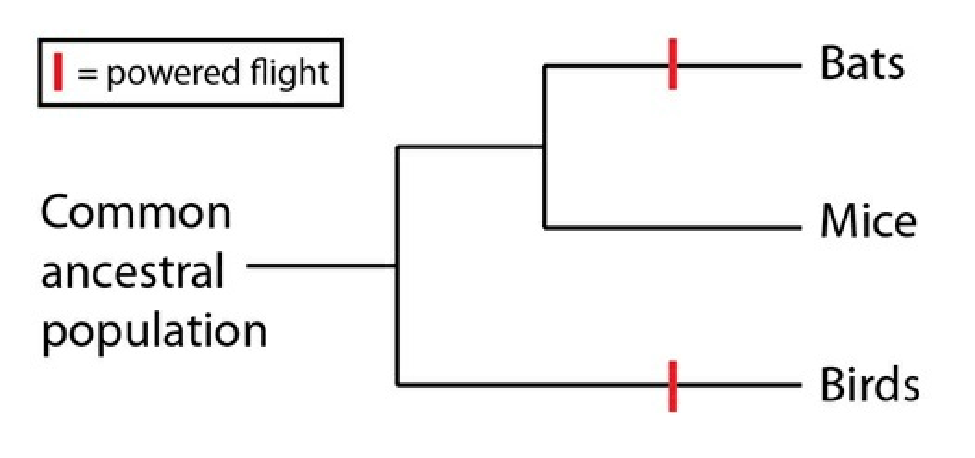
\includegraphics{openbio_files/figure-latex/unnamed-chunk-4-1.pdf}}

\href{https://wp.biologos.org/wp-content/uploads/2018/10/venema_22_7.jpg}{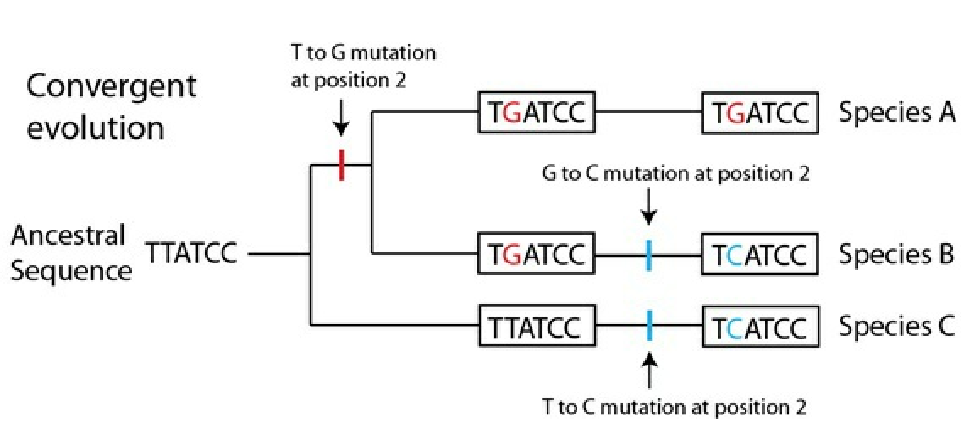
\includegraphics{openbio_files/figure-latex/unnamed-chunk-5-1.pdf}}

\textbf{Derived character}: A character present in one or more species in a clade that was not present in the clade's common ancestor; an evolutionary novelty; also known as an apomorphy. (Contrast with ancestral character)

\textbf{Homologous}: Describes characters derived from a common ancestor. (Contrast with analogous).

\textbf{Homology}: Similarity between species that results from inheritance of traits from a common ancestor. (Contrast with analogy). For more on homologies see \href{https://evolution.berkeley.edu/evolibrary/article/0_0_0/lines_04}{Understanding Evolution: Homologies}, \href{https://evolution.berkeley.edu/evolibrary/article/0_0_0/lines_05}{Homologies: anatomy} , \href{https://evolution.berkeley.edu/evolibrary/article/0_0_0/lines_06}{Homologies: comparative anatomy}, and \href{https://evolution.berkeley.edu/evolibrary/article/0_0_0/lines_07}{Homologies: development} .

\textbf{Homoplasy}: Technical term which indicates similarity in the characters/traits found in different species that are unrelated to common ancestry. Instead, they can be due to convergent evolution or reversal - not common descent. An analogous trait is a type of homoplasy. For an in-depth discussion of homology versus homoplasy see \href{https://www.youtube.com/watch?v=W-APHQ94gog}{this video} (Contrast with homology).

\textbf{Lineage}: A group of ancestral and descendant populations, species, or other taxa that are descended from a common ancestor. Synonymous with clade.

\textbf{Outgroup}: A taxonomic group that diverged prior to the rest of the focal taxa (focal clade) in a phylogenetic analysis.

\textbf{Parsimony}: A criterion for selecting among alternative patterns or explanations based on minimizing the total amount of change or complexity. Can be approximate as ``simpler answers are to be preferred.''

\textbf{Reversal / evolutionary reversal}: An event that results in the reversion of a derived trait (apomorphy) to the ancestral form. This happens frequently at the DNA level, where a mutation can change a base to something different, then later another mutation changes it back. This can be called a back mutation. Reversals can also occur at the protein or morphological level.

\textbf{Trait matrix (aka character matrix, character state matrix, data matrix)}: A table showing the state of each trait occurring in each taxon. Generally, row represents taxa, columns represent characters, and numbers (usually just 0 or 1) represent character states.

\hypertarget{talking-glossary-plasmid-1-min}{%
\section{Talking Glossary: Plasmid (1 min)}\label{talking-glossary-plasmid-1-min}}

National Human Genome Research Institute
\url{https://www.genome.gov/genetics-glossary/Plasmid}

Intro: ``A plasmid is a small, often circular DNA molecule found in bacteria and other cells. Plasmids are separate from the bacterial chromosome and replicate independently of it. They generally carry only a small number of genes, notably some associated with antibiotic resistance. Plasmids may be passed between different bacterial cells.''

Image: \url{https://www.genome.gov/sites/default/files/tg/en/illustration/plasmid.jpg}

Audio: \url{https://www.genome.gov/sites/default/files/tg/en/narration/plasmid.mp3}

Transcription:
``Electrophoresis is a laboratory technique used to separate DNA, RNA, or protein molecules based on their size and electrical charge. An electric current is used to move molecules to be separated through a gel. Pores in the gel work like a sieve, allowing smaller molecules to move faster than larger molecules. The conditions used during electrophoresis can be adjusted to separate molecules in a desired size range.''

\hypertarget{talking-glossary-point-mutation-0.5-min}{%
\section{Talking Glossary: Point mutation (0.5 min)}\label{talking-glossary-point-mutation-0.5-min}}

Point mutation

\url{https://www.genome.gov/genetics-glossary/Point-Mutation}

Abstract: ``A point mutation is when a single base pair is altered. Point mutations can have one of three effects. First, the base substitution can be a silent mutation where the altered codon corresponds to the same amino acid. Second, the base substitution can be a missense mutation where the altered codon corresponds to a different amino acid. Or third, the base substitution can be a nonsense mutation where the altered codon corresponds to a stop signal.''

Image: \url{https://www.genome.gov/sites/default/files/tg/en/illustration/point_mutation.jpg}

Audio: \url{https://www.genome.gov/sites/default/files/tg/en/narration/point_mutation.mp3}

NOTE: Sources vary a little bit in how they define point mutations. Like this glossary entry, I include indels (insertions / deletions) as a type of point mutation.

Transcript:
``Point mutations are a large category of mutations that describe a change in single nucleotide of DNA, such that that nucleotide is switched for another nucleotide, or that nucleotide is deleted, or a single nucleotide is inserted into the DNA that causes that DNA to be different from the normal or wild type gene sequence.

Leslie G. Biesecker, M.D.''

\hypertarget{talking-glossary-polymorphism-1-min}{%
\section{Talking Glossary: Polymorphism (1 min)}\label{talking-glossary-polymorphism-1-min}}

\textbf{Abstract}: ``Polymorphism involves one of two or more variants of a particular DNA sequence {[}and/or protein sequence{]}. The most common type of polymorphism involves variation at a single base pair {[}or amino acid{]}. Polymorphisms can also be much larger in size and involve long stretches of DNA. Called a single nucleotide polymorphism, or SNP (pronounced snip), scientists are studying how SNPs in the human genome correlate with disease, drug response, and other phenotypes.''

\textbf{Transcript}: ``Polymorphism, by strict definitions which hardly anybody pays attention to anymore, is a place in the DNA sequence where there is variation, and the less common variant is present in at least one percent of the people of who you test. That is to distinguish, therefore, polymorphism from a rare variant that might occur in only one in 1,000 people. A polymorphism, it has to occur in at least one in 100 people. Polymorphisms could be not just single-letter changes like a C instead of T. They could also be something more elaborate, like a whole stretch of DNA, that is either present or absent. You might call that a copy number variant; those are all polymorphisms. But this is basically a general term to talk about diversity in genomes in a species.''

Francis S. Collins, M.D., Ph.D.

\hypertarget{talking-glossary-u03-primer-0.5-min}{%
\section{Talking Glossary U03: Primer (0.5 min)}\label{talking-glossary-u03-primer-0.5-min}}

National Human Genome Research Institute

Introduction: ``A primer is a short, single-stranded DNA sequence used in the polymerase chain reaction (PCR) technique. In the PCR method, a pair of primers is used to hybridize with the sample DNA and define the region of the DNA that will be amplified. Primers are also referred to as oligonucleotides.''

Image: \url{https://www.genome.gov/sites/default/files/tg/en/illustration/primer.jpg}

Audio: \url{https://www.genome.gov/sites/default/files/tg/en/narration/primer.mp3}

Transcript
``Primer refers to a small set of nucleotides of DNA, typically 18 to 24 base pairs in length. And a primer can be used for a multitude of other experimental processes. You can use primer in PCR to target a locus to allow for amplification for further analysis. You'd use a primer for sequencing a sequencing reaction where you want to target a very specific region and then do analysis in the extension of that DNA molecule.

\href{https://www.genome.gov/staff/Stacie-Loftus-PhD}{Stacie Loftus}, Ph.D.

\hypertarget{talking-glossary-promoter-1.5-min}{%
\section{Talking Glossary: Promoter (1.5 min)}\label{talking-glossary-promoter-1.5-min}}

\textbf{Abstract}: ``A promoter is a sequence of DNA needed to turn a gene on or off. The process of transcription is initiated at the promoter. Usually found near the beginning of a gene, the promoter has a binding site for the enzyme used to make a messenger RNA (mRNA) molecule.''

\textbf{Audio}: \url{https://www.genome.gov/sites/default/files/tg/en/narration/promoter.mp3}

Image: \url{https://www.genome.gov/sites/default/files/tg/en/illustration/promoter.jpg}

\textbf{Transcript}: ``The promoter region is the sequence typically referred to that's right upstream or right next to where a gene is about to be transcribed. It's the region where certain regulatory elements will bind; these are proteins that will bind to help RNA get transcribed. Now,''promoter'', the term ``promoter'', can actually be a little bit of a nebulous term because it's not very exact. There are specific sequences that are generally found within a promoter region, but sometimes people refer to even extended promoter region that might include sequences that are farther upstream of the gene that might help enhance or repress the particular gene that's about to be transcribed in certain cell types. In general, if you think of the promoter as that piece of DNA that's just upstream of the transcription start site of a gene, that's pretty much what we refer to as promoters.''

Elliott Margulies, Ph.D.

\hypertarget{q}{%
\chapter{Q}\label{q}}

\hypertarget{r}{%
\chapter{R}\label{r}}

\hypertarget{talking-glossary-recessive}{%
\section{Talking Glossary: Recessive}\label{talking-glossary-recessive}}

\url{https://www.genome.gov/genetics-glossary/Recessive}

\textbf{Abstract}: ``Recessive is a quality found in the relationship between two versions of a gene. Individuals receive one version of a gene, called an allele, from each parent. If the alleles are different, the dominant allele will be expressed, while the effect of the other allele, called recessive, is masked. In the case of a recessive genetic disorder, an individual must inherit two copies of the mutated allele in order for the disease to be present.''

Image: \url{https://www.genome.gov/sites/default/files/tg/en/illustration/recessive.jpg}

\textbf{Transcript}: Recessive refers to a type of allele which will not be manifested in an individual unless both of the individual's copies of that gene have that particular genotype. It's usually referred to in conjunction with a Punnett square, other types of Mendelian genetics, and frequently contrasted with a dominant pattern of inheritance wherein if one has one copy of the gene, regardless of what the other copy is, that dominant allele will show itself. In the case of a recessive allele, the individual will show the trait which corresponds to that genotype only if both alleles are the same and have that particular recessive characteristic. Now, that recessive characteristic can be one of no functional consequence. This results in differences between individuals such as in eye color or hair color, but it can also refer to a disease. For instance, in cystic fibrosis, which is a very common Mendelian disorder, that disease exists only when there's a malfunction of both genes that correspond to cystic fibrosis. If there is only one mutation, then that recessive mutation can be compensated for by the normal allele. However, when the function of both are lost, then the disease manifests itself as a recessive disease where there is a loss of function and therefore observable disease.

Christopher P. Austin, M.D.

\hypertarget{talking-glossary-recombinant-dna-0.5-min}{%
\section{Talking Glossary: Recombinant DNA (0.5 min)}\label{talking-glossary-recombinant-dna-0.5-min}}

National Human Genome Research Institute
\url{https://www.genome.gov/genetics-glossary/Recombinant-DNA}

\textbf{Introduction}: ``Recombinant DNA (rDNA) is a technology that uses enzymes to cut and paste together DNA sequences of interest. The recombined DNA sequences can be placed into vehicles called vectors that ferry the DNA into a suitable host cell where it can be copied or expressed.''

Audio: \url{https://www.genome.gov/sites/default/files/tg/en/narration/recombinant_DNA.mp3}

\textbf{Transcript}: ``Pieces of DNA, such as human DNA, can be engineered in a fashion that allows them to be copied, or replicated, in bacteria or yeast. This involves attaching appropriate elements to a piece of DNA and then transferring into a bacterial or yeast cell, with those elements then instructing the bacterial or yeast cell to copy this DNA along with its own. This process is known as DNA cloning, with the resulting cloned DNA often referred to as recombinant DNA.''

\href{https://www.genome.gov/staff/Eric-D-Green-MD-PhD}{Eric D. Green}, M.D., Ph.D.

\hypertarget{talking-glossary-repressor-1-min}{%
\section{Talking Glossary: Repressor (1 min)}\label{talking-glossary-repressor-1-min}}

\textbf{Abstract}: ``A repressor is a protein that turns off the expression of one or more genes. The repressor protein works by binding to the gene's promoter region, preventing the production of messenger RNA (mRNA).''

Audio: \url{https://www.genome.gov/sites/default/files/tg/en/narration/repressor.mp3}

\textbf{Transcript}: ``A repressor is a protein that has a negative effect on gene expression. So these usually are proteins that bind to DNA, and they either prevent the RNA transcription machinery from getting in there and transcribing that DNA, or they just slow it down. So repressors are present in cells where you don't want a particular gene expressed. So if the repressor cell recognizes a sequence in that gene, it will travel to there and keep that gene off in that cell. And this is how you prevent hemoglobin from being expressed in neurons, and how you would prevent liver enzymes from being expressed in red blood cells. Repressors are very difficult to study because it's much easier to study things that give you more of what you're looking for. But I think as we go along we're going to find they play as important a role in gene regulation as the activating proteins.''

David M. Bodine, Ph.D.

\hypertarget{talking-glossary-restriction-enzyme-0.5-min}{%
\section{Talking Glossary: Restriction Enzyme (0.5 min)}\label{talking-glossary-restriction-enzyme-0.5-min}}

National Human Genome Research Institute

\url{https://www.genome.gov/genetics-glossary/Restriction-Enzyme}

Intro: ``A restriction enzyme is an enzyme isolated from bacteria that cuts DNA molecules at specific sequences. The isolation of these enzymes was critical to the development of recombinant DNA (rDNA) technology and genetic engineering.''

Audio: \url{https://www.genome.gov/sites/default/files/tg/en/narration/restriction_enzymes.mp3}

Text ``Restriction enzymes are proteins that bind to DNA in a very specific manner. So they actually recognize the base pairs within the DNA. And typically they will bind to a palindromic sequence, for instance, a sequence that is a mirror copy of itself--AGCCGA.''

\href{https://www.genome.gov/staff/Stacie-Loftus-PhD}{Stacie Loftus}, Ph.D.

\hypertarget{s}{%
\chapter{S}\label{s}}

\hypertarget{talking-glossary-u03-shotgun-sequencing-1-min}{%
\section{Talking Glossary U03: Shotgun sequencing (1 min)}\label{talking-glossary-u03-shotgun-sequencing-1-min}}

Now just called ``sequencing''

\textbf{Introduction}: ``Shotgun sequencing is a laboratory technique for determining the DNA sequence of an organism's genome. The method involves breaking the genome into a collection of small DNA fragments that are sequenced individually. A computer program looks for overlaps in the DNA sequences and uses them to place the individual fragments in their correct order to reconstitute the genome.''

\textbf{Transcript}: ``The most efficient way to sequence a large piece of DNA involves a process known as shotgun sequencing. For this, the starting DNA is broken up randomly into many smaller pieces, sort of in a shotgun fashion, with each of those pieces then sequenced individually. The resulting sequence reads generated from the different pieces are then analyzed by a computer program, looking for stretches of sequence from different reads that are identical with one another. When identical regions are identified, they are overlapped with one another, allowing the two sequence reads to be stitched together. This computer process is repeated over and over and over again, eventually yielding the complete sequence of the starting piece of DNA. The initial random fragmenting and reading of the DNA gave this approach the name''shotgun sequencing''. ''

Eric D. Green, M.D., Ph.D.

\hypertarget{talking-glossary-sickle-cell-disease-4-min}{%
\section{Talking Glossary: Sickle Cell Disease (4 min)}\label{talking-glossary-sickle-cell-disease-4-min}}

\url{https://www.genome.gov/genetics-glossary/Sickle-Cell-Disease}

\textbf{Abstract}: ``Sickle cell disease is a hereditary disease seen most often among people of African ancestry. Caused by mutations in one of the genes that encode the hemoglobin protein, the disease is inherited as an autosomal recessive trait. The mutation causes the red blood cells to take on an unusual sickle shape. Individuals affected by sickle cell disease are chronically anemic and experience significant damage to their heart, lungs, and kidneys.''

Image: \url{https://www.genome.gov/sites/default/files/tg/en/illustration/sickle_cell_disease.jpg}

\textbf{Transcript}: ``Sickle cell disease is the first human inherited disease that was understood at the protein and the DNA level. Sickle cell is a disease that's primarily seen in people of African descent. In studying the genomics of people from Africa, it's very clear now that three different times during the history of the human race the mutation in the beta-globin gene that changes an amino acid at the sixth position of the protein, the same mutation has happened. And this has been expanded throughout history in Africa in three different groups and then migrated all over the world. Now, the mutation does not really affect the ability of beta-globin to participate with alpha-globin and make hemoglobin, and it doesn't affect the ability to carry oxygen. In matter of fact, people who inherit a hemoglobin S gene from their mother and a hemoglobin S gene from their father, so their homozygous for hemoglobin S, have perfectly normal oxygen-carrying capacity of hemoglobin. The problems happen when the red cell containing hemoglobin S gets into the muscles or into your brain and discharges the oxygen. And what happens is that hemoglobin S has a tendency when the oxygen goes off to stick to each other, and they form these polymers. Now, when they get oxygen back on, they go back into solution. The difference between hemoglobin S and wild-type hemoglobin is that the wild-type hemoglobin is soluble when it's got oxygen, and it's also soluble when it doesn't have oxygen. Now, if everything is working well, these polymers in people with sickle cell disease don't get very big. But that can be worsened when you have extreme oxygen stress, and that's what causes the characteristic sickle cells. The polymers get very, very long, and they stretch the cell out of shape. Now your spleen is very good at raking these cells out of the peripheral blood as they come through. And that's what causes the anemia, and the old name for sickle cell was sickle cell anemia. However, though, short polymers are very, very dangerous. If you think of a red blood cell going through your veins and arteries and capillaries as a water balloon, you'll see how it can squish itself down into a long cylinder to get through a capillary and flatten out like a pancake to get through areas in the spleen that kind of rake out the bad-shape red blood cells, and then to form right back to a regular water balloon shape to go into the arteries and veins. But if you have a red blood cell full of these small hemoglobin S polymers, it's like having a water balloon full of ice chips, and as that goes through the capillaries and the small veins, it tears up the lining of these things, just as if you had a cut, and it activates your clotting response and micro-clots will form. And sometimes these get to be bigger and bigger clots, and so the real lethality in sickle cell disease is not from the anemia, it's from this vascular disease. And so it's very unfortunate that about one-third of people who are homozygous for hemoglobin S will have one or more strokes before they're 10 years old. And in those fortunate few that are able to get to be adolescents, these clots can build up in the lungs and give a very severe disease called acute chest syndrome, which is basically emphysema or lung destruction from these obstructions. About one-third of the patients will live healthily to adulthood, but they have many problems with iron-overloaded organs, and their life span is significantly shorter. And it is simply amazing to me that this all comes from one very small change, changes in amino acid, that really isn't having any effect on the normal function of the protein, but has big effects on all of the other systems in the body that the red cells pass through.''

David M. Bodine, Ph.D.

\hypertarget{talking-glossary-somatic-cells-0.75-min}{%
\section{Talking glossary: Somatic cells (0.75 min)}\label{talking-glossary-somatic-cells-0.75-min}}

\url{https://www.genome.gov/genetics-glossary/Somatic-Cells}

\textbf{Abstract}: ``A somatic cell is any cell of the body except sperm and egg cells. Somatic cells are diploid, meaning that they contain two sets of chromosomes, one inherited from each parent. Mutations in somatic cells can affect the individual, but they are not passed on to offspring.''

Image: \url{https://www.genome.gov/sites/default/files/tg/en/illustration/somatic_cells.jpg}

\textbf{Transcript}: ``Somatic cells is a fairly general term which refers to essentially all the cells of the body except for the germ line; the germ line being the cells in the sexual organs that produce sperm and eggs. So anything that doesn't have the job of producing sperm or eggs is a somatic cell. It is very important, of course, for every living organism to be alive, but it contributes nothing in terms of inheritance through genetics, inheritance to the next generation. So it is only of use to the living organism and has no relation to anything that happens in the next generation of that organism.''

Shawn Burgess, Ph.D.

\hypertarget{sequence-annotation}{%
\section{Sequence annotation}\label{sequence-annotation}}

Adapted from Wikipedia, the free encyclopedia

\url{https://en.wikipedia.org/wiki/DNA_annotation}

Note: Wikipedia titles this ``DNA annotation.'' In my experience this phrase is not used; rather we refer to sequence annotation, genome annotation, or just annotation.

Genome annotation is the process of predicting the locations of genes and all of the coding regions in a genome and predicitng what those genes do. An annotation (irrespective of the context) is a note added by way of explanation or commentary. Once a genome is sequenced, it needs to be annotated to make sense of it.{[}1{]}
For DNA annotation, a previously unknown sequence representation of genetic material is enriched with information of intron -exon boundaries, regulatory sequences , gene names and protein products. This annotation is stored in genomic databases.

\hypertarget{process}{%
\subsection{Process}\label{process}}

Genome annotation consists of two main steps:

\begin{enumerate}
\def\labelenumi{\arabic{enumi}.}
\tightlist
\item
  predicting coding elements on the genome , a process called gene prediction
\item
  attaching biological information to these elements
\end{enumerate}

Structural genomic annotation consists of the identification of genomic elements.

\begin{enumerate}
\def\labelenumi{\arabic{enumi}.}
\tightlist
\item
  ORFs {[}open reading frames{]} and their localization
\item
  predicted coding regions
\item
  predicted location of regulatory motifs (e.g.~promoters)
\item
  Functional annotation consists of attaching biological information to genomic elements.
\end{enumerate}

\hypertarget{talking-glossary-substitution-mutation-1.75-min}{%
\section{Talking Glossary: Substitution mutation (1.75 min)}\label{talking-glossary-substitution-mutation-1.75-min}}

\url{https://www.genome.gov/genetics-glossary/Substitution}

\textbf{Abstract}: ``Substitution is a type of mutation where one base pair is replaced by a different base pair. The term also refers to the replacement of one amino acid in a protein with a different amino acid.''

\textbf{Transcript:} ``Subsititution refers to the replacement of one amino acid with another amino acid in a protein or the replacement of one nucleotide with another in DNA or RNA. Substitutions generally give rise to--or they always give rise to--either a polymorphism, that is, a difference between one person, one individual, in a population or another, or a special kind of polymorphism that we call a mutation. In either case, all individuals in the population originally had the same sequence of a gene. There were substitution events that resulted in a change in DNA sequence, which resulted in a change in RNA sequence, which then could result in a change in amino acid sequence. When that happens, that change in DNA sequence or amino acid sequence, or both, could have no effect on the protein, in which case the substitution is benign and has no functional effect. In other cases, if it changes the function of the protein, then it will be observed as either a functional polymorphism, something which increases the effectiveness of the protein product, and therefore would be evolutionarily selected for, or is bad--deleterious--in which case the person might die early and get evolutionarily selected against. Substitutions which lead to mutations, which lead to a deleterious outcome, that is the organism having difficulty with living or dying early, those we call mutations, but they're the result of a certain kind of a substitution.''

Christopher P. Austin, M.D.

\hypertarget{t}{%
\chapter{T}\label{t}}

\hypertarget{taxa-taxon-and-clades-a-brief-primer}{%
\section{Taxa, Taxon, and clades: A Brief Primer}\label{taxa-taxon-and-clades-a-brief-primer}}

By Nathan Brouwer

The following reading discusses what biologists mean when we use the terms taxa, taxon and clade. A few advanced topics are discussed that will be further detailed in future lessons. Names of specific species, families, orders etc. are used as examples; you are not expected to memorize them. A google-doc version of this file can be found here (Links to an external site.).

\textbf{Key Vocab}:
* Taxa
* Taxon
* Clade
* Order
* Taxonomic group
* Primates

\textbf{Advanced topics}:**
* Monophyletic group
* Non-monophyletic group

\hypertarget{what-is-a-taxon}{%
\section{What is a ``taxon''}\label{what-is-a-taxon}}

\textbf{Taxon} and \textbf{clade} refer to different kinds of biological groups. \textbf{Taxa} is the plural of \textbf{taxon}. A taxon (or \textbf{taxonomic group}) can refer to any species \emph{or} group of species. Humans, \emph{Homo sapiens}, is a taxon. We are the genus \emph{Homo}, a larger taxon composed of humans and our close relatives, including Neanderthals (genus: \emph{Homo}, species: \emph{Homo neanderthalensis}). We are part of the \textbf{family} Hominidae, a larger taxon which includes us, chimps and bonobos (genus \emph{Pan}), gorillas (genus \emph{Gorilla}), and orangutans (genus \emph{Pongo}). All primates are part of an \textbf{order}, which includes all the taxa mentioned previously as well as taxa such as monkeys, gibbons, and lemurs. We can say all primates considered together are taxon (a group of species), which is composed of many taxa (many individual species).

The upshot: each level of the hierarchy is a taxon which contains multiple taxa:

\begin{itemize}
\tightlist
\item
  Order: Primates
\item
  Family: Hominidae
\item
  Genus: Homo
\item
  Species: \emph{Homo sapiens}
\end{itemize}

The word ``taxa'' is often used as a generic stand-in for species, family, or order. I can say about my own research ``I studied two taxa of plants'' -- that is, I studied two plant species, though it could also mean I studied two plant families, two plant orders, etc. Someone who studies the phenomena of punctuated equilibrium can say ``the number of taxa on earth increased dramatically during the Cambrian explosion.'' A key way to remember this: Each of the branch tips on a phylogenetic tree is a taxon. Often the tips of a tree are species, but not always.

When using ``taxa'' you don't necessarily have to refer to the current evolutionary or phylogenetic understanding of the species you are talking about. Most taxonomic groups were thought to reflect evolutionary relationships when they were first proposed, but subsequent information has indicated that the group isn't necessarily coherent. For historical reasons and convenience, these taxonomic groups are maintained.

For example, the taxonomic group \textbf{reptiles} includes lizards, snakes, crocodiles, and turtles. These were once thought to be a cohesive group. We now know that birds and crocodiles are \textbf{sister taxa} and that the group we call ``reptiles'' should include birds if it were to be evolutionarily consistent (see \href{https://en.wikipedia.org/wiki/Reptile\#Phylogenetics_and_modern_definition}{here} for a summary). The field known as herpetology focuses on the biology of reptiles, as well as amphibians (frogs and salamanders). This is a group of taxa that excludes birds and evolutionarily isn't coherent. Similarly, the taxonomic group of ``fish'' is problematic from an evolutionary perspective (The precise reasons for this are beyond the scope of this particular reading).

One key point is that ``taxa'' and ``taxon'' do not have to refer to the species level - it could refer to subspecies, populations, or other levels of the hierarchy of biological classification. It is most commonly used in reference to the level of species, but this isn't necessary.

\hypertarget{what-is-a-clade}{%
\section{What is a clade?}\label{what-is-a-clade}}

In contrast to taxon and taxa, \textbf{clade} has a very specific meaning - a clade is \textbf{all} of the taxa that descended from a common ancestor, \emph{plus} the common ancestor. Clade is synonymous with \textbf{monophyletic group}. If you exclude one of the taxa that descended from a common ancestor you end up with what is called a \textbf{non-monophyletic group}. ``Reptiles'' and ``fish'' are taxonomic groups (taxa) that are not clades because they don't contain all of the descendants of their common ancestor and therefore are not evolutionarily coherent.

\textbf{Glossary}:

\begin{itemize}
\tightlist
\item
  Clade -- a group composed of an ancestor and all of its descendants.
\item
  Monophyletic group -- a group composed of an ancestor and all of its descendants (=clade). Example: Reptilia is a monophyletic group if (and only if) it includes birds
\item
  Non-monophyletic group -- a group composed of an ancestor and only some of its descendants, where the missing ones have been placed in another group. Example: ``Reptilia'' is a paraphyletic group if birds are excluded from it. The names of paraphyletic groups are often placed in quotation marks by convention.
\item
  Taxon -- a named group and its constituent members. Normally a taxon will be a named clade. Phylogenetic definition (of a group) -- a definition for a group that is based on common ancestry. Example 1: Tetrapoda is the group composed of the last common ancestor of living amphibians and amniotes and all taxa more closely related to that clade than to lungfish.
\end{itemize}

\hypertarget{further-reading}{%
\section{Further Reading:}\label{further-reading}}

For more on clades: \url{http://en.wikipedia.org/wiki/Clade}
For more on taxa: \url{https://en.wikipedia.org/wiki/Taxon}

``In biology, a taxon (plural taxa), from taxonomy, is a group of one or more populations of an organism or organisms seen by taxonomists to form a unit.''
ICZN (1999) International Code of Zoological Nomenclature.

``A taxonomic unit, whether named or not: i.e.~a population, or group of populations of organisms which are usually inferred to be phylogenetically related and which have characters in common which differentiate (q.v.) the unit (e.g.~a geographic population, a genus, a family, an order) from other such units.''

For information on non-monophyletic groups and why fish aren't a clade, see these sites

\begin{itemize}
\tightlist
\item
  \url{http://ess17.blogspot.com/2008/06/q-can-you-please-explain-question-3-on.html}
\item
  \url{https://en.wikipedia.org/wiki/Paraphyly}
\item
  \url{https://en.wikipedia.org/wiki/Fish}
\end{itemize}

\hypertarget{talking-glossary-trait-0.75-min}{%
\section{Talking Glossary: Trait (0.75 min)}\label{talking-glossary-trait-0.75-min}}

Abstract: ``A trait is a specific characteristic of an organism. Traits can be determined by genes or the environment, or more commonly by interactions between them. The genetic contribution to a trait is called the genotype. The outward expression of the genotype is called the phenotype.''

Comments:
In ecology and evolutionary biology, we often use the terms trait and character interchangeably. In phylogenetics the term character is common.

In phylogenetics, we organize our data in a grid called a trait matrix, or a character matrix. We can consider phenotypic traits/phenotypic characters or sequences (genetic traits/genetic characters). Often we refer to phenotypic traits as morphological traits if they have to do with the size, shape, structure, anatomy etc. of an organism.

The definition here in the Talking Glossary highlights the fact that phenotypic traits are due to both genes and the environment. When we do phylogenetics with phenotypic traits we strive to use consistent morphological differences that are due to genetics. Because phenotypic traits like height, weight, color etc can vary so much due to the environment we use traits that can take on distinct states, like tails: monkeys have tails while humans don't; dogs long have tails but bears have very short ones. We therefore draw a distinction between characters (e.g.~tails) and character states (tail present, tail absent).

Audio: \url{https://www.genome.gov/sites/default/files/tg/en/narration/trait.mp3}

Transcript
``Trait is a specific characteristic of an individual. For example, their hair color or their blood type. Traits are determined by genes, and also they are determined by the interaction with the environment with genes. And remember that genes are the messages in our DNA that define individual characteristics. So the trait is the manifestation of the product of a gene that is coded for by the DNA. The word''phenotype'' is sometimes used interchangeably with the word trait, and ``phenotype'' may also define a whole compendium of traits together.''

\href{https://www.nigms.nih.gov/about/Pages/krasnewich.aspx}{Donna Krasnewich}, M.D., Ph.D.~Program director in the Division of \href{https://www.nigms.nih.gov/about/overview/Pages/GMCDB.aspx}{Genetics and Molecular, Cellular, and Developmental Biology}, National Institutes of Health

Photograph: \url{https://www.nigms.nih.gov/about/PublishingImages/headshots/headshot-donna-krasnewich-small.jpg}

\hypertarget{u}{%
\chapter{U}\label{u}}

\hypertarget{v}{%
\chapter{V}\label{v}}

\hypertarget{talking-glossary-vector-2-min}{%
\section{Talking Glossary: Vector (2 min)}\label{talking-glossary-vector-2-min}}

National Human Genome Research Institute

Note: Usually refers to a plasmid, though in this entry they mention how it can also apply to viruses.

Introduction: ``A vector is any vehicle, often a virus or a plasmid {[}usually a plasmid in practice, and that's what we focus on in this class{]} that is used to ferry a desired DNA sequence into a host cell as part of a molecular cloning procedure. Depending on the purpose of the cloning procedure, the vector may assist in multiplying, isolating, or expressing the foreign DNA insert.''

Audio: \url{https://www.genome.gov/sites/default/files/tg/en/narration/vector.mp3}

Transcript
``A vector is a way to take a sequence of DNA, usually, and introduce it into another place. So what vectors do is allow you to propagate the DNA you're interested in, in the organism you've chosen to propagate it in. So the simplest one is the origins of recombinant DNA technology: They made copies of RNAs, and they were able to insert these into what is known as plasmids. Now, plasmids are kind of mini-bacterial chromosomes. They have a way to replicate themselves, and what makes it work is they also carry one or two genes on them that make them resistant to specific antibiotics. So if you can insert the gene you're interested in into this plasmid, you can select for the bacteria that have picked up that plasmid by growing them on an antibiotic that, if they haven't picked it up, would kill them. So that plasmid is a vector for taking a particular DNA sequence into a bacteria. And then you can isolate one colony of bacteria and clone that, grow that clone up, and that's how you would propagate that. There are other vectors that are larger and will have multiple sites of origins of replication, and these are known as bacterial artificial chromosomes, and they can handle much larger pieces of DNA. There are yeast artificial chromosomes that allow very large fragments of DNA to be grown in yeast cells. And recently, human artificial chromosome have been developed that allow enormous pieces of DNA to be introduced and propagated into human cells. So vector is really just a means to take a piece of DNA that you're interested in and insert it, and select for it, and identify it in the organism that you want to propagate it in.''

\href{https://www.genome.gov/staff/David-M-Bodine-PhD}{David M. Bodine}, Ph.D

\hypertarget{w}{%
\chapter{W}\label{w}}

\hypertarget{talking-glossary-x-chromosome-1.25-min}{%
\section{Talking Glossary: X-chromosome (1.25 min)}\label{talking-glossary-x-chromosome-1.25-min}}

Length: 1.25 min

\url{https://www.genome.gov/genetics-glossary/X-Chromosome}

Abstract: The X chromosome is one of two sex chromosomes. Humans and most mammals have two sex chromosomes, the X and Y. Some individuals have two X chromosomes in their cells, while others have X and Y chromosomes in their cells. Egg cells all contain an X chromosome, while sperm cells contain an X or a Y chromosome. This arrangement means that during fertilization, it is the XY parent that determines the whether the offspring will be XY or XX.

Image: \url{https://www.genome.gov/sites/default/files/tg/en/illustration/x_chromosome.jpg}

Audio: \url{https://www.genome.gov/sites/default/files/tg/en/narration/x-chromosome.mp3}

Transcript
``So this, because I'm a female, is truly one of my favorite chromosomes. As you know, females have two X chromosomes. They're quite large in comparison to the male chromosomes. They are carried by the egg, and so consequently you pass on--if you have an egg--you can only pass on an X chromosome to your offspring. What's also quite interesting is the number of genes that are found on the X chromosome. It is predicted that there are approximately 155 million base pairs, which translates to about 900 to 1,400 genes on the X chromosome. Meaning that it carries about five percent of the total DNA in the entire cell. Which is quite in contrast to the Y chromosome, which is considerably smaller. Again, if you look at the X chromosomes in the genes that it carries, often times you'll see that sex-linked disorders are carried on the X chromosome. Which is why, as I stated before, they're more predominant in male, because there's not a protective mechanism against having a mutation on one of those genes because we don't have the normal copy of that gene on the X chromosome.''

Carla Easter, Ph.D.

Image: \url{https://www.genome.gov/sites/default/files/genome-old/images/content/easter_carla.jpg}

Biography

Carla Easter, Ph.D., is chief of the Education and Community Involvement Branch at the National Human Genome Research Institute (NHGRI). She played a major role in the development of the NHGRI/Smithsonian exhibition Genome: Unlocking Life's Code, and its accompanying website, and serves as a liaison to the K-12 and university community as a speaker on genomic science and career preparation and pathways. Dr.~Easter also serves as an adjunct faculty member at the University of the District of Columbia Department of Biology, Chemistry and Physics.

From 2003-2006, Dr.~Easter was director of outreach for Washington University School of Medicine's Genome Sequencing Center. Before assuming her role as outreach director, Dr.~Easter was a research associate in the Department of Education at Washington University (2001-2003) where she explored the notions of science among secondary students. She served as pre-college coordinator for the NASA Summer High School Apprenticeship Research Plus Program and project associate for the Quality Education for Minorities Network. From 1997-2000, Dr.~Easter conducted post-doctoral research at Washington University School of Medicine on the virulence factors associated with Streptococcus pyogenes.

Dr.~Easter earned her bachelor's degree in microbiology from the University of California, Los Angeles and her doctoral in biology with an emphasis on molecular genetics from the University of California, San Diego.

Video: \url{https://youtu.be/S1-Y8cO-sMc}
Dr.~Easter is a laboratory scientist who now specializes in science communication and outreach. The video below is a discussion between Dr.~Easter and a highschool student sponsored by the Children's Science Center Lab

The YouTube video below contains an audio-only interview with Dr.~Easter
\url{https://youtu.be/X_CX7FWSfoM}

\hypertarget{talking-glossary-x-inactivation-lyonization-1.45-min}{%
\section{Talking Glossary: X-inactivation (``Lyonization''; 1.45 min))}\label{talking-glossary-x-inactivation-lyonization-1.45-min}}

\url{https://www.genome.gov/genetics-glossary/Lyonization} (Links to an external site.)

Abstract: ``Lyonization is commonly known as X-inactivation. In mammals, males receive one copy of the X chromosome while females receive two copies. To prevent female cells from having twice as many gene products from the X chromosomes as males, one copy of the X chromosome in each female cell is inactivated. In placental mammals, the choice of which X chromosome is inactivated is random, whereas in marsupials it is always the paternal copy that is inactivated.''

Audio

Transcript: ``Lyonization is named after Mary Lyon, who was a geneticist who first figured out that in females who have two copies of the X chromosome, that one copy of each gene is turned off permanently in one chromosome or another. So that females, who have two copies of the X chromosome, and males, who have one copy of the X chromosome, are both human, and they can both operate fairly normally. So this process of turning off one copy of one gene or another on the X chromosome is called lyonization, and it happens from a series of essentially irreversible chemical modifications to one copy of the gene. The fascinating thing about this is that in so-called X-linked diseases, if the female inherits a gene responsible for an X-linked disease, and has one copy that's abnormal and one copy that's normal, the abnormal gene is almost always the one that's turned off. And the normal gene is almost always allowed to stay on. In X-linked diseases in males, of course, X-linked diseases manifest because they only have one X chromosome, and so those mutated genes have to show up. But the fascinating part about it, which we really don't understand, is how it is that the body knows if the female inherits one copy of a gene that is abnormal and would otherwise cause an X-linked disease if the normal copy was lyonized and turned off. That doesn't happen. The abnormal copy gets turned off, leaving the normal copy to function, and saving the female from having the disease.''

Christopher P. Austin, M.D.

History:

English geneticist Mary Lyons (\url{https://en.wikipedia.org/wiki/Mary_F._Lyon}) first characterized X-inactivation. You can read a short article about her life here (\url{https://www.nature.com/articles/518036a}).

\hypertarget{x}{%
\chapter{X}\label{x}}

\hypertarget{v-1}{%
\chapter{V}\label{v-1}}

\hypertarget{additional-glossaries}{%
\section{Additional Glossaries}\label{additional-glossaries}}

\url{https://www.ncbi.nlm.nih.gov/books/NBK5191/}

\hypertarget{z}{%
\chapter{Z}\label{z}}

\end{document}
